% Options for packages loaded elsewhere
\PassOptionsToPackage{unicode}{hyperref}
\PassOptionsToPackage{hyphens}{url}
\PassOptionsToPackage{space}{xeCJK}
%
\documentclass[
]{article}
\usepackage{amsmath,amssymb}
\usepackage{iftex}
\ifPDFTeX
  \usepackage[T1]{fontenc}
  \usepackage[utf8]{inputenc}
  \usepackage{textcomp} % provide euro and other symbols
\else % if luatex or xetex
  \usepackage{unicode-math} % this also loads fontspec
  \defaultfontfeatures{Scale=MatchLowercase}
  \defaultfontfeatures[\rmfamily]{Ligatures=TeX,Scale=1}
\fi
\usepackage{lmodern}
\ifPDFTeX\else
  % xetex/luatex font selection
  \ifXeTeX
    \usepackage{xeCJK}
    \setCJKmainfont[]{SimSun}
          \fi
  \ifLuaTeX
    \usepackage[]{luatexja-fontspec}
    \setmainjfont[]{SimSun}
  \fi
\fi
% Use upquote if available, for straight quotes in verbatim environments
\IfFileExists{upquote.sty}{\usepackage{upquote}}{}
\IfFileExists{microtype.sty}{% use microtype if available
  \usepackage[]{microtype}
  \UseMicrotypeSet[protrusion]{basicmath} % disable protrusion for tt fonts
}{}
\makeatletter
\@ifundefined{KOMAClassName}{% if non-KOMA class
  \IfFileExists{parskip.sty}{%
    \usepackage{parskip}
  }{% else
    \setlength{\parindent}{0pt}
    \setlength{\parskip}{6pt plus 2pt minus 1pt}}
}{% if KOMA class
  \KOMAoptions{parskip=half}}
\makeatother
\usepackage{xcolor}
\usepackage[margin=1in]{geometry}
\usepackage{color}
\usepackage{fancyvrb}
\newcommand{\VerbBar}{|}
\newcommand{\VERB}{\Verb[commandchars=\\\{\}]}
\DefineVerbatimEnvironment{Highlighting}{Verbatim}{commandchars=\\\{\}}
% Add ',fontsize=\small' for more characters per line
\usepackage{framed}
\definecolor{shadecolor}{RGB}{248,248,248}
\newenvironment{Shaded}{\begin{snugshade}}{\end{snugshade}}
\newcommand{\AlertTok}[1]{\textcolor[rgb]{0.94,0.16,0.16}{#1}}
\newcommand{\AnnotationTok}[1]{\textcolor[rgb]{0.56,0.35,0.01}{\textbf{\textit{#1}}}}
\newcommand{\AttributeTok}[1]{\textcolor[rgb]{0.13,0.29,0.53}{#1}}
\newcommand{\BaseNTok}[1]{\textcolor[rgb]{0.00,0.00,0.81}{#1}}
\newcommand{\BuiltInTok}[1]{#1}
\newcommand{\CharTok}[1]{\textcolor[rgb]{0.31,0.60,0.02}{#1}}
\newcommand{\CommentTok}[1]{\textcolor[rgb]{0.56,0.35,0.01}{\textit{#1}}}
\newcommand{\CommentVarTok}[1]{\textcolor[rgb]{0.56,0.35,0.01}{\textbf{\textit{#1}}}}
\newcommand{\ConstantTok}[1]{\textcolor[rgb]{0.56,0.35,0.01}{#1}}
\newcommand{\ControlFlowTok}[1]{\textcolor[rgb]{0.13,0.29,0.53}{\textbf{#1}}}
\newcommand{\DataTypeTok}[1]{\textcolor[rgb]{0.13,0.29,0.53}{#1}}
\newcommand{\DecValTok}[1]{\textcolor[rgb]{0.00,0.00,0.81}{#1}}
\newcommand{\DocumentationTok}[1]{\textcolor[rgb]{0.56,0.35,0.01}{\textbf{\textit{#1}}}}
\newcommand{\ErrorTok}[1]{\textcolor[rgb]{0.64,0.00,0.00}{\textbf{#1}}}
\newcommand{\ExtensionTok}[1]{#1}
\newcommand{\FloatTok}[1]{\textcolor[rgb]{0.00,0.00,0.81}{#1}}
\newcommand{\FunctionTok}[1]{\textcolor[rgb]{0.13,0.29,0.53}{\textbf{#1}}}
\newcommand{\ImportTok}[1]{#1}
\newcommand{\InformationTok}[1]{\textcolor[rgb]{0.56,0.35,0.01}{\textbf{\textit{#1}}}}
\newcommand{\KeywordTok}[1]{\textcolor[rgb]{0.13,0.29,0.53}{\textbf{#1}}}
\newcommand{\NormalTok}[1]{#1}
\newcommand{\OperatorTok}[1]{\textcolor[rgb]{0.81,0.36,0.00}{\textbf{#1}}}
\newcommand{\OtherTok}[1]{\textcolor[rgb]{0.56,0.35,0.01}{#1}}
\newcommand{\PreprocessorTok}[1]{\textcolor[rgb]{0.56,0.35,0.01}{\textit{#1}}}
\newcommand{\RegionMarkerTok}[1]{#1}
\newcommand{\SpecialCharTok}[1]{\textcolor[rgb]{0.81,0.36,0.00}{\textbf{#1}}}
\newcommand{\SpecialStringTok}[1]{\textcolor[rgb]{0.31,0.60,0.02}{#1}}
\newcommand{\StringTok}[1]{\textcolor[rgb]{0.31,0.60,0.02}{#1}}
\newcommand{\VariableTok}[1]{\textcolor[rgb]{0.00,0.00,0.00}{#1}}
\newcommand{\VerbatimStringTok}[1]{\textcolor[rgb]{0.31,0.60,0.02}{#1}}
\newcommand{\WarningTok}[1]{\textcolor[rgb]{0.56,0.35,0.01}{\textbf{\textit{#1}}}}
\usepackage{longtable,booktabs,array}
\usepackage{calc} % for calculating minipage widths
% Correct order of tables after \paragraph or \subparagraph
\usepackage{etoolbox}
\makeatletter
\patchcmd\longtable{\par}{\if@noskipsec\mbox{}\fi\par}{}{}
\makeatother
% Allow footnotes in longtable head/foot
\IfFileExists{footnotehyper.sty}{\usepackage{footnotehyper}}{\usepackage{footnote}}
\makesavenoteenv{longtable}
\usepackage{graphicx}
\makeatletter
\def\maxwidth{\ifdim\Gin@nat@width>\linewidth\linewidth\else\Gin@nat@width\fi}
\def\maxheight{\ifdim\Gin@nat@height>\textheight\textheight\else\Gin@nat@height\fi}
\makeatother
% Scale images if necessary, so that they will not overflow the page
% margins by default, and it is still possible to overwrite the defaults
% using explicit options in \includegraphics[width, height, ...]{}
\setkeys{Gin}{width=\maxwidth,height=\maxheight,keepaspectratio}
% Set default figure placement to htbp
\makeatletter
\def\fps@figure{htbp}
\makeatother
\setlength{\emergencystretch}{3em} % prevent overfull lines
\providecommand{\tightlist}{%
  \setlength{\itemsep}{0pt}\setlength{\parskip}{0pt}}
\setcounter{secnumdepth}{5}
\ifLuaTeX
  \usepackage{selnolig}  % disable illegal ligatures
\fi
\IfFileExists{bookmark.sty}{\usepackage{bookmark}}{\usepackage{hyperref}}
\IfFileExists{xurl.sty}{\usepackage{xurl}}{} % add URL line breaks if available
\urlstyle{same}
\hypersetup{
  pdftitle={时间序列分析第三章作业},
  pdfauthor={Phlinsia},
  hidelinks,
  pdfcreator={LaTeX via pandoc}}

\title{时间序列分析第三章作业}
\author{Phlinsia}
\date{2024年3月25日}

\begin{document}
\maketitle

{
\setcounter{tocdepth}{2}
\tableofcontents
}
\hypertarget{ux5e73ux5747ux5de5ux4f5cux65f6ux95f4}{%
\subsection{3.4 平均工作时间}\label{ux5e73ux5747ux5de5ux4f5cux65f6ux95f4}}

\hypertarget{a}{%
\subsubsection*{a}\label{a}}
\addcontentsline{toc}{subsubsection}{a}

\begin{Shaded}
\begin{Highlighting}[]
\FunctionTok{library}\NormalTok{(TSA)}
\FunctionTok{data}\NormalTok{(}\StringTok{"hours"}\NormalTok{)}
\FunctionTok{xyplot}\NormalTok{(hours,}\AttributeTok{xlab=}\StringTok{"时间"}\NormalTok{)}
\end{Highlighting}
\end{Shaded}

\begin{figure}
\centering
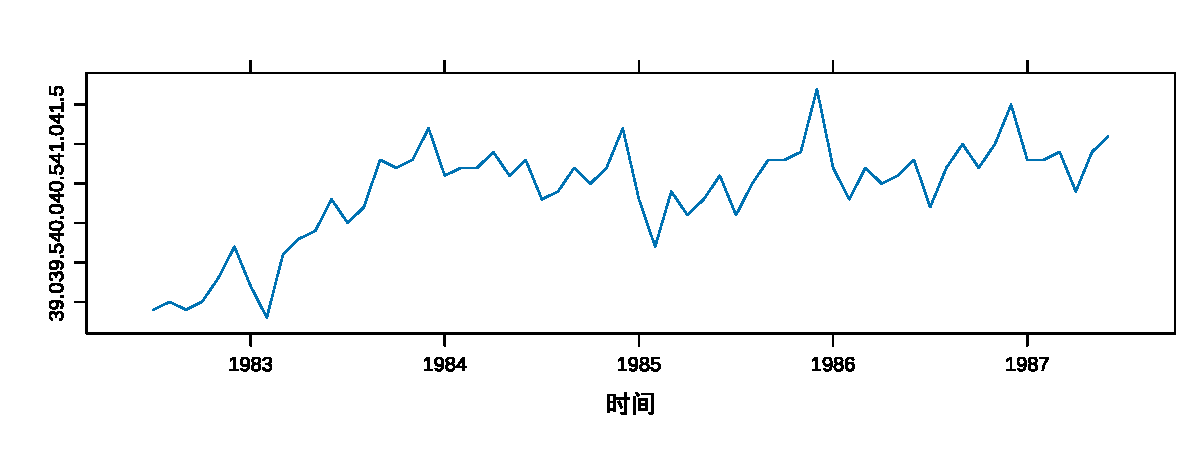
\includegraphics{chapter3_files/figure-latex/unnamed-chunk-1-1.pdf}
\caption{\label{fig:unnamed-chunk-1}美国制造业每周平均工作时间的月度数值}
\end{figure}

在图1中,可见83年到84年间有急剧增长。此外,存在季节性趋势:一般来说,后半年的工作时间较长,除了夏季;不过84年并没有明显的模式。

\hypertarget{b}{%
\subsubsection*{b}\label{b}}
\addcontentsline{toc}{subsubsection}{b}

\begin{Shaded}
\begin{Highlighting}[]
\NormalTok{months }\OtherTok{\textless{}{-}} \FunctionTok{c}\NormalTok{(}\StringTok{"J"}\NormalTok{, }\StringTok{"A"}\NormalTok{, }\StringTok{"S"}\NormalTok{, }\StringTok{"O"}\NormalTok{, }\StringTok{"N"}\NormalTok{, }\StringTok{"D"}\NormalTok{, }\StringTok{"J"}\NormalTok{, }\StringTok{"F"}\NormalTok{, }\StringTok{"M"}\NormalTok{, }\StringTok{"A"}\NormalTok{, }\StringTok{"M"}\NormalTok{, }\StringTok{"J"}\NormalTok{)}

\FunctionTok{xyplot}\NormalTok{(hours, }\AttributeTok{panel =} \ControlFlowTok{function}\NormalTok{(x, y, ...) \{}
  \FunctionTok{panel.xyplot}\NormalTok{(x, y, ...)}
  \FunctionTok{panel.text}\NormalTok{(}\AttributeTok{x =}\NormalTok{ x, }\AttributeTok{y =}\NormalTok{ y, }\AttributeTok{labels =}\NormalTok{ months)}
\NormalTok{\}, }\AttributeTok{xlab =} \StringTok{"时间"}\NormalTok{)}
\end{Highlighting}
\end{Shaded}

\begin{figure}
\centering
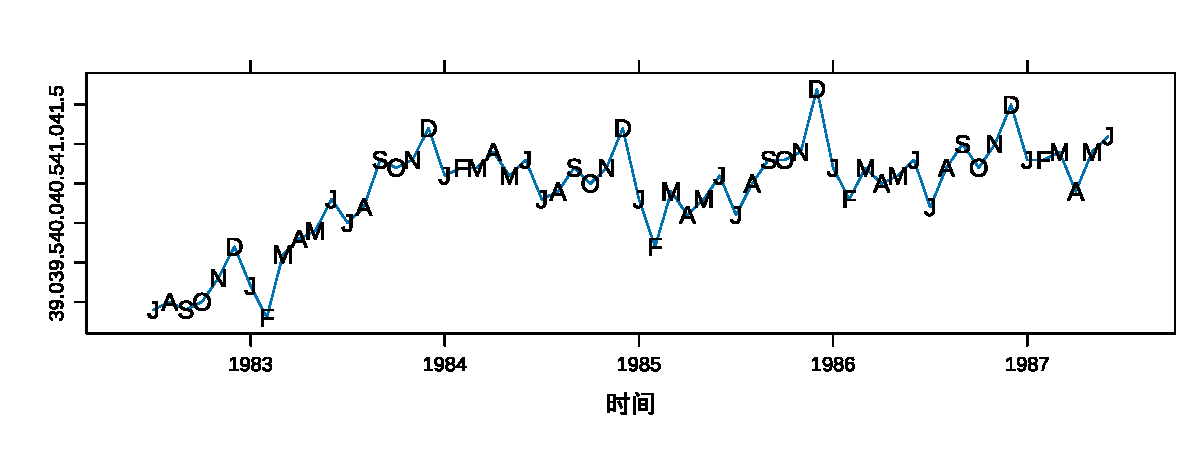
\includegraphics{chapter3_files/figure-latex/unnamed-chunk-2-1.pdf}
\caption{\label{fig:unnamed-chunk-2}每周平均工作时间的月度数值(标注月份)}
\end{figure}

在图2中,我们的解释基本相同。12月是每周工作时间最长的月份,而2月和1月是最短的,趋势显而易见。

\hypertarget{ux5de5ux8d44}{%
\subsection{3.5 工资}\label{ux5de5ux8d44}}

\hypertarget{a-1}{%
\subsubsection*{a}\label{a-1}}
\addcontentsline{toc}{subsubsection}{a}

\begin{Shaded}
\begin{Highlighting}[]
\FunctionTok{data}\NormalTok{(}\StringTok{"wages"}\NormalTok{)}
\FunctionTok{xyplot}\NormalTok{(wages, }\AttributeTok{panel =} \ControlFlowTok{function}\NormalTok{(x, y, ...) \{}
  \FunctionTok{panel.xyplot}\NormalTok{(x, y, ...)}
  \FunctionTok{panel.text}\NormalTok{(x, y, }\AttributeTok{labels =}\NormalTok{ months)}
\NormalTok{\}, }\AttributeTok{xlab =} \StringTok{"时间"}\NormalTok{)}
\end{Highlighting}
\end{Shaded}

\begin{figure}
\centering
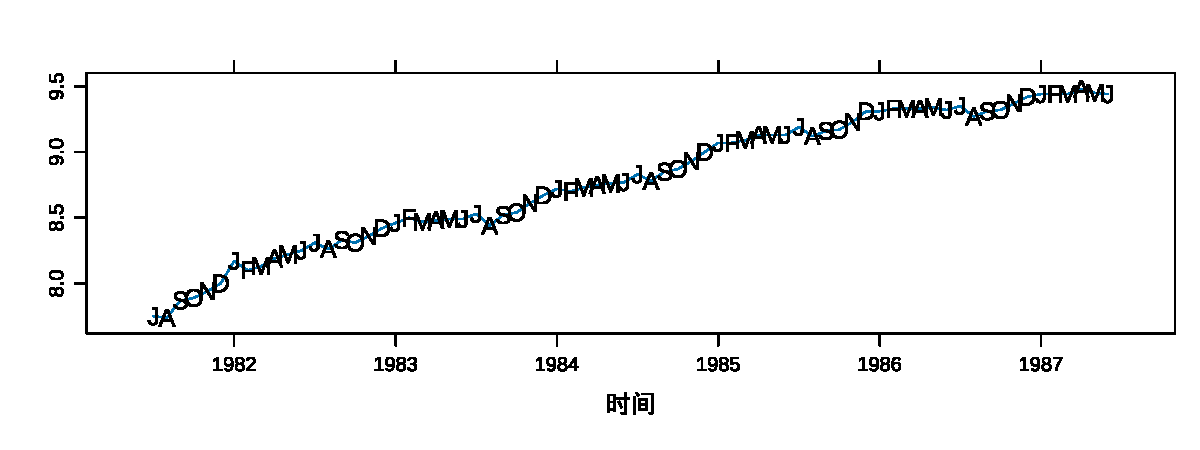
\includegraphics{chapter3_files/figure-latex/unnamed-chunk-3-1.pdf}
\caption{\label{fig:unnamed-chunk-3}美国服装和纺织业工人每月平均小时工资。}
\end{figure}

工资呈现出一个季节性的正向趋势:8月是工资的低谷。
一般来说,秋季的增长似乎更大。

\hypertarget{b-1}{%
\subsubsection*{b}\label{b-1}}
\addcontentsline{toc}{subsubsection}{b}

\begin{Shaded}
\begin{Highlighting}[]
\NormalTok{wages\_fit1 }\OtherTok{\textless{}{-}} \FunctionTok{lm}\NormalTok{(wages }\SpecialCharTok{\textasciitilde{}} \FunctionTok{time}\NormalTok{(wages))}
\FunctionTok{summary}\NormalTok{(wages\_fit1)}
\end{Highlighting}
\end{Shaded}

\begin{verbatim}
## 
## Call:
## lm(formula = wages ~ time(wages))
## 
## Residuals:
##      Min       1Q   Median       3Q      Max 
## -0.23828 -0.04981  0.01942  0.05845  0.13136 
## 
## Coefficients:
##               Estimate Std. Error t value Pr(>|t|)    
## (Intercept) -5.490e+02  1.115e+01  -49.24   <2e-16 ***
## time(wages)  2.811e-01  5.618e-03   50.03   <2e-16 ***
## ---
## Signif. codes:  0 '***' 0.001 '**' 0.01 '*' 0.05 '.' 0.1 ' ' 1
## 
## Residual standard error: 0.08257 on 70 degrees of freedom
## Multiple R-squared:  0.9728, Adjusted R-squared:  0.9724 
## F-statistic:  2503 on 1 and 70 DF,  p-value: < 2.2e-16
\end{verbatim}

\begin{Shaded}
\begin{Highlighting}[]
\NormalTok{wages\_rst }\OtherTok{\textless{}{-}} \FunctionTok{rstudent}\NormalTok{(wages\_fit1)}
\end{Highlighting}
\end{Shaded}

\hypertarget{c}{%
\subsubsection*{c}\label{c}}
\addcontentsline{toc}{subsubsection}{c}

\begin{Shaded}
\begin{Highlighting}[]
\FunctionTok{xyplot}\NormalTok{(wages\_rst }\SpecialCharTok{\textasciitilde{}} \FunctionTok{time}\NormalTok{(wages\_rst), }\AttributeTok{type =} \StringTok{"l"}\NormalTok{,}
       \AttributeTok{xlab =} \StringTok{"时间"}\NormalTok{, }\AttributeTok{ylab =} \StringTok{"学生化残差"}\NormalTok{)}
\end{Highlighting}
\end{Shaded}

\begin{figure}
\centering
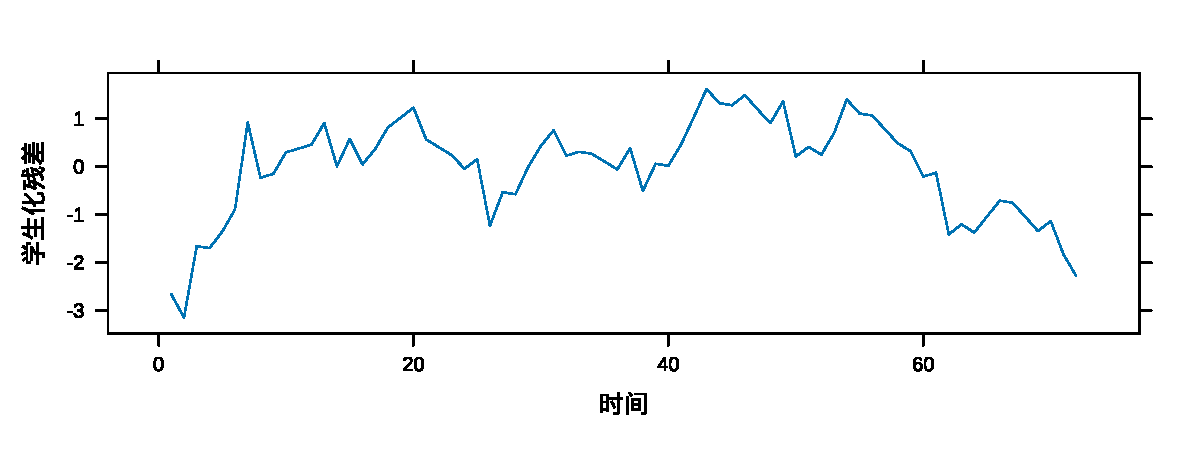
\includegraphics{chapter3_files/figure-latex/wages-resid-1.pdf}
\caption{\label{fig:wages-resid}残差图}
\end{figure}

此时似乎仍然存在与时间相关的自相关性,而不是白噪声。

\hypertarget{d}{%
\subsubsection*{d}\label{d}}
\addcontentsline{toc}{subsubsection}{d}

\begin{Shaded}
\begin{Highlighting}[]
\NormalTok{wages\_fit2 }\OtherTok{\textless{}{-}} \FunctionTok{lm}\NormalTok{(wages }\SpecialCharTok{\textasciitilde{}} \FunctionTok{time}\NormalTok{(wages) }\SpecialCharTok{+} \FunctionTok{I}\NormalTok{(}\FunctionTok{time}\NormalTok{(wages)}\SpecialCharTok{\^{}}\DecValTok{2}\NormalTok{))}
\FunctionTok{summary}\NormalTok{(wages\_fit2)}
\end{Highlighting}
\end{Shaded}

\begin{verbatim}
## 
## Call:
## lm(formula = wages ~ time(wages) + I(time(wages)^2))
## 
## Residuals:
##       Min        1Q    Median        3Q       Max 
## -0.148318 -0.041440  0.001563  0.050089  0.139839 
## 
## Coefficients:
##                    Estimate Std. Error t value Pr(>|t|)    
## (Intercept)      -8.495e+04  1.019e+04  -8.336 4.87e-12 ***
## time(wages)       8.534e+01  1.027e+01   8.309 5.44e-12 ***
## I(time(wages)^2) -2.143e-02  2.588e-03  -8.282 6.10e-12 ***
## ---
## Signif. codes:  0 '***' 0.001 '**' 0.01 '*' 0.05 '.' 0.1 ' ' 1
## 
## Residual standard error: 0.05889 on 69 degrees of freedom
## Multiple R-squared:  0.9864, Adjusted R-squared:  0.986 
## F-statistic:  2494 on 2 and 69 DF,  p-value: < 2.2e-16
\end{verbatim}

\begin{Shaded}
\begin{Highlighting}[]
\NormalTok{wages\_rst2 }\OtherTok{\textless{}{-}} \FunctionTok{rstudent}\NormalTok{(wages\_fit2)}
\end{Highlighting}
\end{Shaded}

\hypertarget{e}{%
\subsubsection*{e}\label{e}}
\addcontentsline{toc}{subsubsection}{e}

\begin{Shaded}
\begin{Highlighting}[]
\FunctionTok{xyplot}\NormalTok{(wages\_rst2 }\SpecialCharTok{\textasciitilde{}} \FunctionTok{time}\NormalTok{(wages\_rst), }\AttributeTok{type =} \StringTok{"l"}\NormalTok{,}
       \AttributeTok{xlab =} \StringTok{"时间"}\NormalTok{, }\AttributeTok{ylab =} \StringTok{"学生化残差"}\NormalTok{)}
\end{Highlighting}
\end{Shaded}

\begin{figure}
\centering
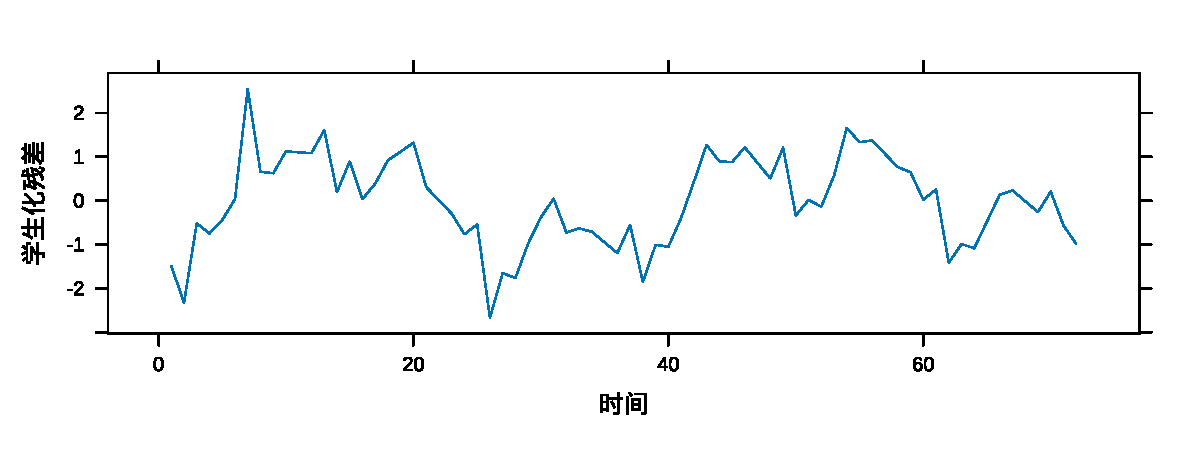
\includegraphics{chapter3_files/figure-latex/wages_quad_resid-1.pdf}
\caption{(\#fig:wages\_quad\_resid)我们二次模型的残差图}
\end{figure}

像随机噪声,但拟合残差之间的自相关性仍清晰,这是我们尚未在模型中捕捉到的。

\hypertarget{ux5564ux9152ux9500ux552e}{%
\subsection{3.6 啤酒销售}\label{ux5564ux9152ux9500ux552e}}

\hypertarget{a-2}{%
\subsubsection*{a}\label{a-2}}
\addcontentsline{toc}{subsubsection}{a}

\begin{Shaded}
\begin{Highlighting}[]
\FunctionTok{data}\NormalTok{(beersales)}
\FunctionTok{xyplot}\NormalTok{(beersales,}\AttributeTok{xlab=}\StringTok{"时间"}\NormalTok{)}
\end{Highlighting}
\end{Shaded}

\begin{figure}
\centering
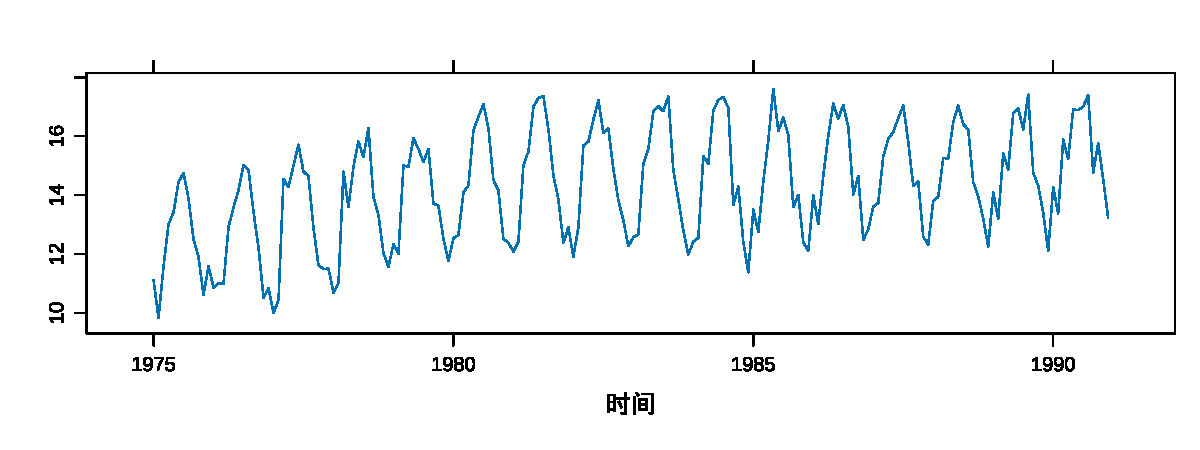
\includegraphics{chapter3_files/figure-latex/unnamed-chunk-6-1.pdf}
\caption{\label{fig:unnamed-chunk-6}美国啤酒月销售额。}
\end{figure}

清晰的季节性趋势。75年到81年左右有个初始的正向趋势,然后趋于稳定。

\hypertarget{b-2}{%
\subsubsection*{b}\label{b-2}}
\addcontentsline{toc}{subsubsection}{b}

\begin{Shaded}
\begin{Highlighting}[]
\NormalTok{months }\OtherTok{\textless{}{-}} \FunctionTok{c}\NormalTok{(}\StringTok{"J"}\NormalTok{, }\StringTok{"F"}\NormalTok{, }\StringTok{"M"}\NormalTok{, }\StringTok{"A"}\NormalTok{, }\StringTok{"M"}\NormalTok{, }\StringTok{"J"}\NormalTok{, }\StringTok{"J"}\NormalTok{, }\StringTok{"A"}\NormalTok{, }\StringTok{"S"}\NormalTok{, }\StringTok{"O"}\NormalTok{, }\StringTok{"N"}\NormalTok{, }\StringTok{"D"}\NormalTok{)}

\FunctionTok{xyplot}\NormalTok{(beersales,}
       \AttributeTok{panel =} \ControlFlowTok{function}\NormalTok{(x, y, ...) \{}
         \FunctionTok{panel.xyplot}\NormalTok{(x, y, ...)}
         \FunctionTok{panel.text}\NormalTok{(x, y, }\AttributeTok{labels =}\NormalTok{ months)}
\NormalTok{       \},}\AttributeTok{xlab=}\StringTok{"时间"}\NormalTok{)}
\end{Highlighting}
\end{Shaded}

\begin{figure}
\centering
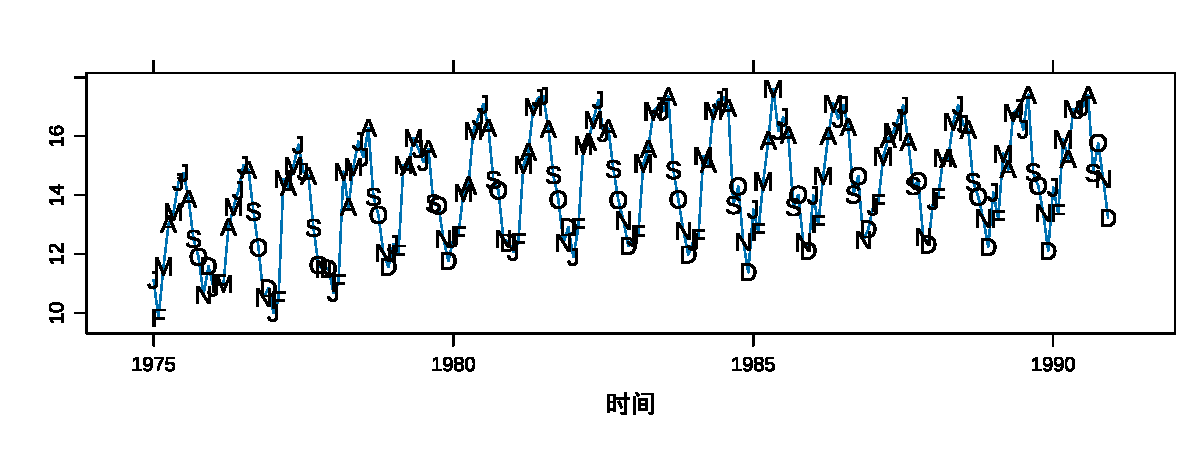
\includegraphics{chapter3_files/figure-latex/unnamed-chunk-7-1.pdf}
\caption{\label{fig:unnamed-chunk-7}带有月份首字母标注的美国啤酒月销售额。}
\end{figure}

明显可见销售高峰在暖和的月份,而秋冬季则低迷。12月特别低,而5月、6月和7月似乎是高峰期。

\hypertarget{c-1}{%
\subsubsection*{c}\label{c-1}}
\addcontentsline{toc}{subsubsection}{c}

\begin{Shaded}
\begin{Highlighting}[]
\NormalTok{beer\_fit1 }\OtherTok{\textless{}{-}} \FunctionTok{lm}\NormalTok{(beersales }\SpecialCharTok{\textasciitilde{}} \FunctionTok{season}\NormalTok{(beersales))}
\FunctionTok{pander}\NormalTok{(}\FunctionTok{summary}\NormalTok{(beer\_fit1))}
\end{Highlighting}
\end{Shaded}

\begin{longtable}[]{@{}
  >{\centering\arraybackslash}p{(\columnwidth - 8\tabcolsep) * \real{0.4125}}
  >{\centering\arraybackslash}p{(\columnwidth - 8\tabcolsep) * \real{0.1375}}
  >{\centering\arraybackslash}p{(\columnwidth - 8\tabcolsep) * \real{0.1625}}
  >{\centering\arraybackslash}p{(\columnwidth - 8\tabcolsep) * \real{0.1250}}
  >{\centering\arraybackslash}p{(\columnwidth - 8\tabcolsep) * \real{0.1625}}@{}}
\toprule\noalign{}
\begin{minipage}[b]{\linewidth}\centering
~
\end{minipage} & \begin{minipage}[b]{\linewidth}\centering
Estimate
\end{minipage} & \begin{minipage}[b]{\linewidth}\centering
Std. Error
\end{minipage} & \begin{minipage}[b]{\linewidth}\centering
t value
\end{minipage} & \begin{minipage}[b]{\linewidth}\centering
Pr(\textgreater\textbar t\textbar)
\end{minipage} \\
\midrule\noalign{}
\endhead
\bottomrule\noalign{}
\endlastfoot
\textbf{(Intercept)} & 12.49 & 0.2639 & 47.31 & 1.786e-103 \\
\textbf{season(beersales)February} & -0.1426 & 0.3732 & -0.382 & 0.7029 \\
\textbf{season(beersales)March} & 2.082 & 0.3732 & 5.579 & 8.771e-08 \\
\textbf{season(beersales)April} & 2.398 & 0.3732 & 6.424 & 1.151e-09 \\
\textbf{season(beersales)May} & 3.599 & 0.3732 & 9.643 & 5.322e-18 \\
\textbf{season(beersales)June} & 3.85 & 0.3732 & 10.31 & 6.813e-20 \\
\textbf{season(beersales)July} & 3.769 & 0.3732 & 10.1 & 2.812e-19 \\
\textbf{season(beersales)August} & 3.609 & 0.3732 & 9.669 & 4.494e-18 \\
\textbf{season(beersales)September} & 1.573 & 0.3732 & 4.214 & 3.964e-05 \\
\textbf{season(beersales)October} & 1.254 & 0.3732 & 3.361 & 0.0009484 \\
\textbf{season(beersales)November} & -0.04797 & 0.3732 & -0.1285 & 0.8979 \\
\textbf{season(beersales)December} & -0.4231 & 0.3732 & -1.134 & 0.2585 \\
\end{longtable}

\begin{longtable}[]{@{}
  >{\centering\arraybackslash}p{(\columnwidth - 6\tabcolsep) * \real{0.2083}}
  >{\centering\arraybackslash}p{(\columnwidth - 6\tabcolsep) * \real{0.3056}}
  >{\centering\arraybackslash}p{(\columnwidth - 6\tabcolsep) * \real{0.1250}}
  >{\centering\arraybackslash}p{(\columnwidth - 6\tabcolsep) * \real{0.2361}}@{}}
\caption{Fitting linear model: beersales \textasciitilde{} season(beersales)}\tabularnewline
\toprule\noalign{}
\begin{minipage}[b]{\linewidth}\centering
Observations
\end{minipage} & \begin{minipage}[b]{\linewidth}\centering
Residual Std. Error
\end{minipage} & \begin{minipage}[b]{\linewidth}\centering
\(R^2\)
\end{minipage} & \begin{minipage}[b]{\linewidth}\centering
Adjusted \(R^2\)
\end{minipage} \\
\midrule\noalign{}
\endfirsthead
\toprule\noalign{}
\begin{minipage}[b]{\linewidth}\centering
Observations
\end{minipage} & \begin{minipage}[b]{\linewidth}\centering
Residual Std. Error
\end{minipage} & \begin{minipage}[b]{\linewidth}\centering
\(R^2\)
\end{minipage} & \begin{minipage}[b]{\linewidth}\centering
Adjusted \(R^2\)
\end{minipage} \\
\midrule\noalign{}
\endhead
\bottomrule\noalign{}
\endlastfoot
192 & 1.056 & 0.7103 & 0.6926 \\
\end{longtable}

所有比较都是相对1月份来的。这个模型解释了大约0.71的方差,并且在统计上显著。大多数因素都显著(主要是冬季月份,如预期所示)。

\hypertarget{d-1}{%
\subsubsection*{d}\label{d-1}}
\addcontentsline{toc}{subsubsection}{d}

\begin{Shaded}
\begin{Highlighting}[]
\FunctionTok{xyplot}\NormalTok{(}\FunctionTok{rstudent}\NormalTok{(beer\_fit1) }\SpecialCharTok{\textasciitilde{}} \FunctionTok{time}\NormalTok{(beersales), }\AttributeTok{type =} \StringTok{"l"}\NormalTok{,}
       \AttributeTok{xlab =} \StringTok{"时间"}\NormalTok{, }\AttributeTok{ylab =} \StringTok{"学生化残差"}\NormalTok{,}
       \AttributeTok{panel =} \ControlFlowTok{function}\NormalTok{(x, y, ...) \{}
         \FunctionTok{panel.xyplot}\NormalTok{(x, y, ...)}
         \FunctionTok{panel.xyplot}\NormalTok{(x, y, }\AttributeTok{pch =} \FunctionTok{as.vector}\NormalTok{(}\FunctionTok{season}\NormalTok{(beersales)), }\AttributeTok{col =} \DecValTok{1}\NormalTok{)}
\NormalTok{       \})}
\end{Highlighting}
\end{Shaded}

\begin{figure}
\centering
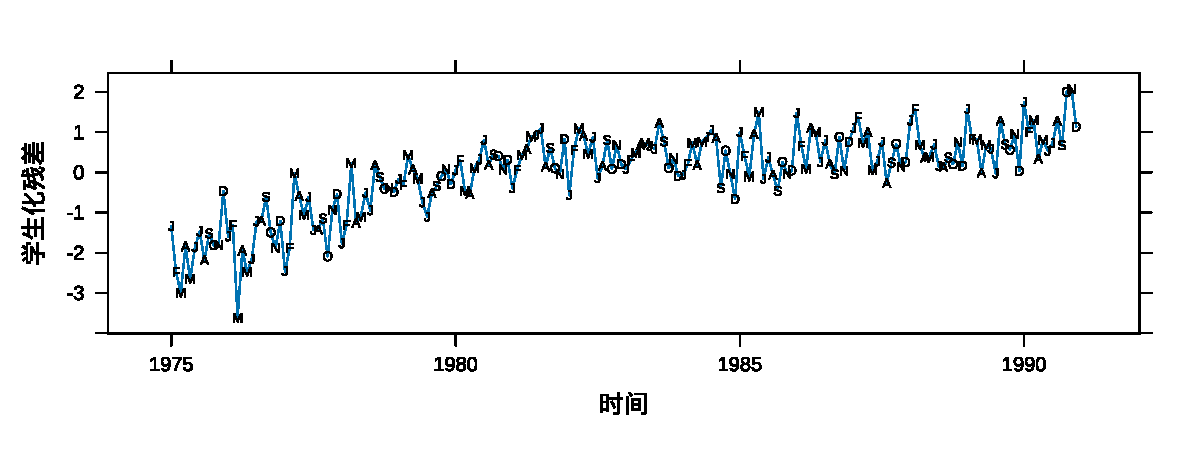
\includegraphics{chapter3_files/figure-latex/rst-beer-1.pdf}
\caption{\label{fig:rst-beer}啤酒销售残差图。}
\end{figure}

观察残差图,在 \ref{fig:rst-beer} 中我们没能很好地拟合数据;我们没捕捉到长期趋势。

\hypertarget{e-1}{%
\subsubsection*{e}\label{e-1}}
\addcontentsline{toc}{subsubsection}{e}

\begin{Shaded}
\begin{Highlighting}[]
\NormalTok{beer\_fit2 }\OtherTok{\textless{}{-}} \FunctionTok{lm}\NormalTok{(beersales }\SpecialCharTok{\textasciitilde{}} \FunctionTok{season}\NormalTok{(beersales) }\SpecialCharTok{+} \FunctionTok{time}\NormalTok{(beersales) }\SpecialCharTok{+}
                  \FunctionTok{I}\NormalTok{(}\FunctionTok{time}\NormalTok{(beersales) }\SpecialCharTok{\^{}} \DecValTok{2}\NormalTok{))}
\FunctionTok{pander}\NormalTok{(}\FunctionTok{summary}\NormalTok{(beer\_fit2))}
\end{Highlighting}
\end{Shaded}

\begin{longtable}[]{@{}
  >{\centering\arraybackslash}p{(\columnwidth - 8\tabcolsep) * \real{0.4177}}
  >{\centering\arraybackslash}p{(\columnwidth - 8\tabcolsep) * \real{0.1392}}
  >{\centering\arraybackslash}p{(\columnwidth - 8\tabcolsep) * \real{0.1646}}
  >{\centering\arraybackslash}p{(\columnwidth - 8\tabcolsep) * \real{0.1266}}
  >{\centering\arraybackslash}p{(\columnwidth - 8\tabcolsep) * \real{0.1519}}@{}}
\toprule\noalign{}
\begin{minipage}[b]{\linewidth}\centering
~
\end{minipage} & \begin{minipage}[b]{\linewidth}\centering
Estimate
\end{minipage} & \begin{minipage}[b]{\linewidth}\centering
Std. Error
\end{minipage} & \begin{minipage}[b]{\linewidth}\centering
t value
\end{minipage} & \begin{minipage}[b]{\linewidth}\centering
Pr(\textgreater\textbar t\textbar)
\end{minipage} \\
\midrule\noalign{}
\endhead
\bottomrule\noalign{}
\endlastfoot
\textbf{(Intercept)} & -71498 & 8791 & -8.133 & 6.932e-14 \\
\textbf{season(beersales)February} & -0.1579 & 0.209 & -0.7554 & 0.451 \\
\textbf{season(beersales)March} & 2.052 & 0.209 & 9.818 & 1.864e-18 \\
\textbf{season(beersales)April} & 2.353 & 0.209 & 11.26 & 1.533e-22 \\
\textbf{season(beersales)May} & 3.539 & 0.209 & 16.93 & 6.063e-39 \\
\textbf{season(beersales)June} & 3.776 & 0.209 & 18.06 & 4.117e-42 \\
\textbf{season(beersales)July} & 3.681 & 0.209 & 17.61 & 7.706e-41 \\
\textbf{season(beersales)August} & 3.507 & 0.2091 & 16.78 & 1.698e-38 \\
\textbf{season(beersales)September} & 1.458 & 0.2091 & 6.972 & 5.89e-11 \\
\textbf{season(beersales)October} & 1.126 & 0.2091 & 5.385 & 2.268e-07 \\
\textbf{season(beersales)November} & -0.1894 & 0.2091 & -0.9059 & 0.3662 \\
\textbf{season(beersales)December} & -0.5773 & 0.2092 & -2.76 & 0.00638 \\
\textbf{time(beersales)} & 71.96 & 8.867 & 8.115 & 7.703e-14 \\
\textbf{I(time(beersales)\^{}2)} & -0.0181 & 0.002236 & -8.096 & 8.633e-14 \\
\end{longtable}

\begin{longtable}[]{@{}
  >{\centering\arraybackslash}p{(\columnwidth - 6\tabcolsep) * \real{0.2083}}
  >{\centering\arraybackslash}p{(\columnwidth - 6\tabcolsep) * \real{0.3056}}
  >{\centering\arraybackslash}p{(\columnwidth - 6\tabcolsep) * \real{0.1250}}
  >{\centering\arraybackslash}p{(\columnwidth - 6\tabcolsep) * \real{0.2361}}@{}}
\caption{Fitting linear model: beersales \textasciitilde{} season(beersales) + time(beersales) + I(time(beersales)\^{}2)}\tabularnewline
\toprule\noalign{}
\begin{minipage}[b]{\linewidth}\centering
Observations
\end{minipage} & \begin{minipage}[b]{\linewidth}\centering
Residual Std. Error
\end{minipage} & \begin{minipage}[b]{\linewidth}\centering
\(R^2\)
\end{minipage} & \begin{minipage}[b]{\linewidth}\centering
Adjusted \(R^2\)
\end{minipage} \\
\midrule\noalign{}
\endfirsthead
\toprule\noalign{}
\begin{minipage}[b]{\linewidth}\centering
Observations
\end{minipage} & \begin{minipage}[b]{\linewidth}\centering
Residual Std. Error
\end{minipage} & \begin{minipage}[b]{\linewidth}\centering
\(R^2\)
\end{minipage} & \begin{minipage}[b]{\linewidth}\centering
Adjusted \(R^2\)
\end{minipage} \\
\midrule\noalign{}
\endhead
\bottomrule\noalign{}
\endlastfoot
192 & 0.5911 & 0.9102 & 0.9036 \\
\end{longtable}

这个模型更好地拟合了数据,解释了大约0.91的方差。

\hypertarget{f}{%
\subsubsection*{f}\label{f}}
\addcontentsline{toc}{subsubsection}{f}

\begin{Shaded}
\begin{Highlighting}[]
\FunctionTok{xyplot}\NormalTok{(}\FunctionTok{rstudent}\NormalTok{(beer\_fit2) }\SpecialCharTok{\textasciitilde{}} \FunctionTok{time}\NormalTok{(beersales), }\AttributeTok{type =} \StringTok{"l"}\NormalTok{,}
       \AttributeTok{xlab =} \StringTok{"时间"}\NormalTok{, }\AttributeTok{yla =} \StringTok{"学生化残差"}\NormalTok{,}
       \AttributeTok{panel =} \ControlFlowTok{function}\NormalTok{(x, y, ...) \{}
         \FunctionTok{panel.xyplot}\NormalTok{(x, y, ...)}
         \FunctionTok{panel.xyplot}\NormalTok{(x, y, }\AttributeTok{pch =} \FunctionTok{as.vector}\NormalTok{(}\FunctionTok{season}\NormalTok{(beersales)), }\AttributeTok{col =} \DecValTok{1}\NormalTok{)}
\NormalTok{       \})}
\end{Highlighting}
\end{Shaded}

\begin{figure}
\centering
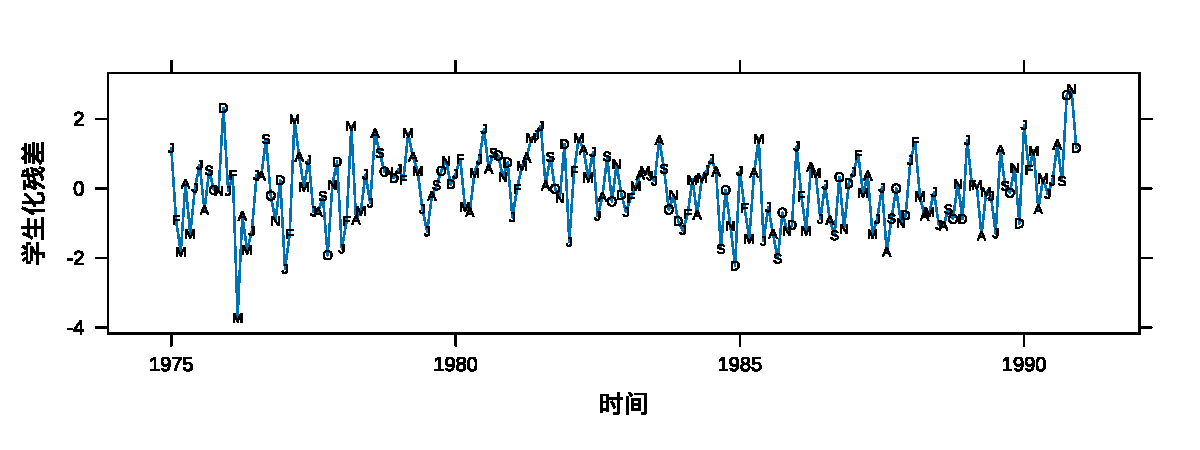
\includegraphics{chapter3_files/figure-latex/rst-beer2-1.pdf}
\caption{\label{fig:rst-beer2}二次拟合的啤酒销售残差图。}
\end{figure}

许多值仍无法成功预测,但我们现在能更好地建模长期趋势。

\hypertarget{ux6e29ux5c3cux8d1dux6208ux623fux8f66ux9500ux552eux6570ux636eux5206ux6790}{%
\subsection{3.7 温尼贝戈房车销售数据分析}\label{ux6e29ux5c3cux8d1dux6208ux623fux8f66ux9500ux552eux6570ux636eux5206ux6790}}

\hypertarget{a-3}{%
\subsubsection*{a}\label{a-3}}
\addcontentsline{toc}{subsubsection}{a}

\begin{Shaded}
\begin{Highlighting}[]
\FunctionTok{data}\NormalTok{(winnebago)}
\FunctionTok{xyplot}\NormalTok{(winnebago,}\AttributeTok{xlab=}\StringTok{"时间"}\NormalTok{)}
\end{Highlighting}
\end{Shaded}

\begin{figure}
\centering
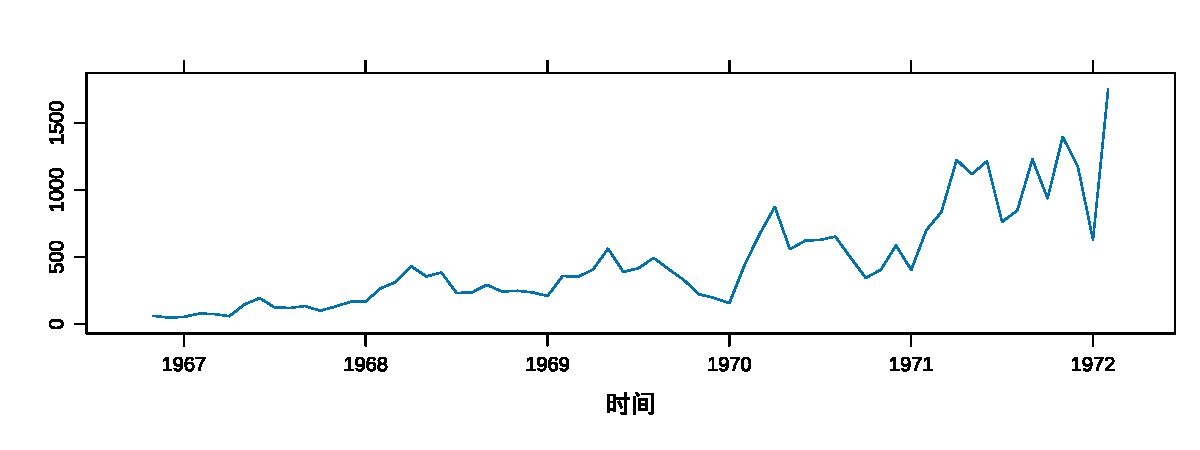
\includegraphics{chapter3_files/figure-latex/winnebago-1.pdf}
\caption{\label{fig:winnebago}温尼贝戈房车每月单位销售量图。}
\end{figure}

\hypertarget{b-3}{%
\subsubsection*{b}\label{b-3}}
\addcontentsline{toc}{subsubsection}{b}

\begin{Shaded}
\begin{Highlighting}[]
\NormalTok{winn\_fit1 }\OtherTok{\textless{}{-}} \FunctionTok{lm}\NormalTok{(winnebago }\SpecialCharTok{\textasciitilde{}} \FunctionTok{time}\NormalTok{(winnebago))}
\FunctionTok{pander}\NormalTok{(}\FunctionTok{summary}\NormalTok{(winn\_fit1))}
\end{Highlighting}
\end{Shaded}

\begin{longtable}[]{@{}
  >{\centering\arraybackslash}p{(\columnwidth - 8\tabcolsep) * \real{0.3056}}
  >{\centering\arraybackslash}p{(\columnwidth - 8\tabcolsep) * \real{0.1528}}
  >{\centering\arraybackslash}p{(\columnwidth - 8\tabcolsep) * \real{0.1806}}
  >{\centering\arraybackslash}p{(\columnwidth - 8\tabcolsep) * \real{0.1389}}
  >{\centering\arraybackslash}p{(\columnwidth - 8\tabcolsep) * \real{0.1667}}@{}}
\toprule\noalign{}
\begin{minipage}[b]{\linewidth}\centering
~
\end{minipage} & \begin{minipage}[b]{\linewidth}\centering
Estimate
\end{minipage} & \begin{minipage}[b]{\linewidth}\centering
Std. Error
\end{minipage} & \begin{minipage}[b]{\linewidth}\centering
t value
\end{minipage} & \begin{minipage}[b]{\linewidth}\centering
Pr(\textgreater\textbar t\textbar)
\end{minipage} \\
\midrule\noalign{}
\endhead
\bottomrule\noalign{}
\endlastfoot
\textbf{(Intercept)} & -394886 & 33540 & -11.77 & 1.87e-17 \\
\textbf{time(winnebago)} & 200.7 & 17.03 & 11.79 & 1.777e-17 \\
\end{longtable}

\begin{longtable}[]{@{}
  >{\centering\arraybackslash}p{(\columnwidth - 6\tabcolsep) * \real{0.2083}}
  >{\centering\arraybackslash}p{(\columnwidth - 6\tabcolsep) * \real{0.3056}}
  >{\centering\arraybackslash}p{(\columnwidth - 6\tabcolsep) * \real{0.1250}}
  >{\centering\arraybackslash}p{(\columnwidth - 6\tabcolsep) * \real{0.2361}}@{}}
\caption{Fitting linear model: winnebago \textasciitilde{} time(winnebago)}\tabularnewline
\toprule\noalign{}
\begin{minipage}[b]{\linewidth}\centering
Observations
\end{minipage} & \begin{minipage}[b]{\linewidth}\centering
Residual Std. Error
\end{minipage} & \begin{minipage}[b]{\linewidth}\centering
\(R^2\)
\end{minipage} & \begin{minipage}[b]{\linewidth}\centering
Adjusted \(R^2\)
\end{minipage} \\
\midrule\noalign{}
\endfirsthead
\toprule\noalign{}
\begin{minipage}[b]{\linewidth}\centering
Observations
\end{minipage} & \begin{minipage}[b]{\linewidth}\centering
Residual Std. Error
\end{minipage} & \begin{minipage}[b]{\linewidth}\centering
\(R^2\)
\end{minipage} & \begin{minipage}[b]{\linewidth}\centering
Adjusted \(R^2\)
\end{minipage} \\
\midrule\noalign{}
\endhead
\bottomrule\noalign{}
\endlastfoot
64 & 209.7 & 0.6915 & 0.6865 \\
\end{longtable}

该模型具有显著性,并解释了0.69的方差。

\begin{Shaded}
\begin{Highlighting}[]
\FunctionTok{xyplot}\NormalTok{(}\FunctionTok{rstudent}\NormalTok{(winn\_fit1) }\SpecialCharTok{\textasciitilde{}} \FunctionTok{time}\NormalTok{(winnebago), }\AttributeTok{type =} \StringTok{"l"}\NormalTok{,}
       \AttributeTok{xlab =} \StringTok{"时间"}\NormalTok{, }\AttributeTok{ylab =} \StringTok{"学生化残差"}\NormalTok{)}
\end{Highlighting}
\end{Shaded}

\begin{figure}
\centering
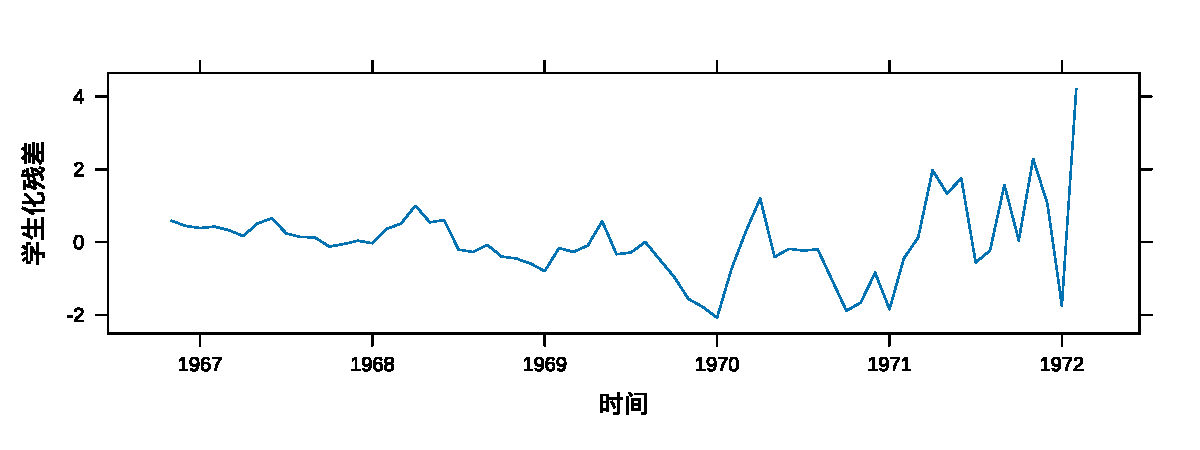
\includegraphics{chapter3_files/figure-latex/winnebago-lm-res-1.pdf}
\caption{\label{fig:winnebago-lm-res}温尼贝戈房车数据线性拟合残差图。}
\end{figure}

该拟合效果较差(图\ref{fig:winnebago-lm-res})。残差分布并非随机,并且明显看出对于后期年份我们的预测准确性更差。

\hypertarget{c-2}{%
\subsubsection*{c}\label{c-2}}
\addcontentsline{toc}{subsubsection}{c}

为了更好拟合,我们对结果变量采用自然对数变换。

\begin{Shaded}
\begin{Highlighting}[]
\NormalTok{winn\_fit\_log }\OtherTok{\textless{}{-}} \FunctionTok{lm}\NormalTok{(}\FunctionTok{log}\NormalTok{(winnebago) }\SpecialCharTok{\textasciitilde{}} \FunctionTok{time}\NormalTok{(winnebago))}
\FunctionTok{pander}\NormalTok{(}\FunctionTok{summary}\NormalTok{(winn\_fit\_log))}
\end{Highlighting}
\end{Shaded}

\begin{longtable}[]{@{}
  >{\centering\arraybackslash}p{(\columnwidth - 8\tabcolsep) * \real{0.3056}}
  >{\centering\arraybackslash}p{(\columnwidth - 8\tabcolsep) * \real{0.1528}}
  >{\centering\arraybackslash}p{(\columnwidth - 8\tabcolsep) * \real{0.1806}}
  >{\centering\arraybackslash}p{(\columnwidth - 8\tabcolsep) * \real{0.1389}}
  >{\centering\arraybackslash}p{(\columnwidth - 8\tabcolsep) * \real{0.1667}}@{}}
\toprule\noalign{}
\begin{minipage}[b]{\linewidth}\centering
~
\end{minipage} & \begin{minipage}[b]{\linewidth}\centering
Estimate
\end{minipage} & \begin{minipage}[b]{\linewidth}\centering
Std. Error
\end{minipage} & \begin{minipage}[b]{\linewidth}\centering
t value
\end{minipage} & \begin{minipage}[b]{\linewidth}\centering
Pr(\textgreater\textbar t\textbar)
\end{minipage} \\
\midrule\noalign{}
\endhead
\bottomrule\noalign{}
\endlastfoot
\textbf{(Intercept)} & -984.9 & 62.99 & -15.64 & 3.45e-23 \\
\textbf{time(winnebago)} & 0.5031 & 0.03199 & 15.73 & 2.575e-23 \\
\end{longtable}

\begin{longtable}[]{@{}
  >{\centering\arraybackslash}p{(\columnwidth - 6\tabcolsep) * \real{0.2083}}
  >{\centering\arraybackslash}p{(\columnwidth - 6\tabcolsep) * \real{0.3056}}
  >{\centering\arraybackslash}p{(\columnwidth - 6\tabcolsep) * \real{0.1250}}
  >{\centering\arraybackslash}p{(\columnwidth - 6\tabcolsep) * \real{0.2361}}@{}}
\caption{Fitting linear model: log(winnebago) \textasciitilde{} time(winnebago)}\tabularnewline
\toprule\noalign{}
\begin{minipage}[b]{\linewidth}\centering
Observations
\end{minipage} & \begin{minipage}[b]{\linewidth}\centering
Residual Std. Error
\end{minipage} & \begin{minipage}[b]{\linewidth}\centering
\(R^2\)
\end{minipage} & \begin{minipage}[b]{\linewidth}\centering
Adjusted \(R^2\)
\end{minipage} \\
\midrule\noalign{}
\endfirsthead
\toprule\noalign{}
\begin{minipage}[b]{\linewidth}\centering
Observations
\end{minipage} & \begin{minipage}[b]{\linewidth}\centering
Residual Std. Error
\end{minipage} & \begin{minipage}[b]{\linewidth}\centering
\(R^2\)
\end{minipage} & \begin{minipage}[b]{\linewidth}\centering
Adjusted \(R^2\)
\end{minipage} \\
\midrule\noalign{}
\endhead
\bottomrule\noalign{}
\endlastfoot
64 & 0.3939 & 0.7996 & 0.7964 \\
\end{longtable}

变换后模型改善,解释了近0.8的方差。

\hypertarget{d-2}{%
\subsubsection*{d}\label{d-2}}
\addcontentsline{toc}{subsubsection}{d}

\begin{Shaded}
\begin{Highlighting}[]
\FunctionTok{xyplot}\NormalTok{(}\FunctionTok{rstudent}\NormalTok{(winn\_fit\_log) }\SpecialCharTok{\textasciitilde{}} \FunctionTok{time}\NormalTok{(winnebago), }\AttributeTok{type =} \StringTok{"l"}\NormalTok{,}
       \AttributeTok{xlab =} \StringTok{"时间"}\NormalTok{, }\AttributeTok{ylab =} \StringTok{"学生化残差"}\NormalTok{,}
       \AttributeTok{panel =} \ControlFlowTok{function}\NormalTok{(x, y, ...) \{}
         \FunctionTok{panel.xyplot}\NormalTok{(x, y, ...)}
         \FunctionTok{panel.xyplot}\NormalTok{(x, y, }\AttributeTok{pch =} \FunctionTok{as.vector}\NormalTok{(}\FunctionTok{season}\NormalTok{(winnebago)), }\AttributeTok{col =} \DecValTok{1}\NormalTok{)}
\NormalTok{       \})}
\end{Highlighting}
\end{Shaded}

\begin{figure}
\centering
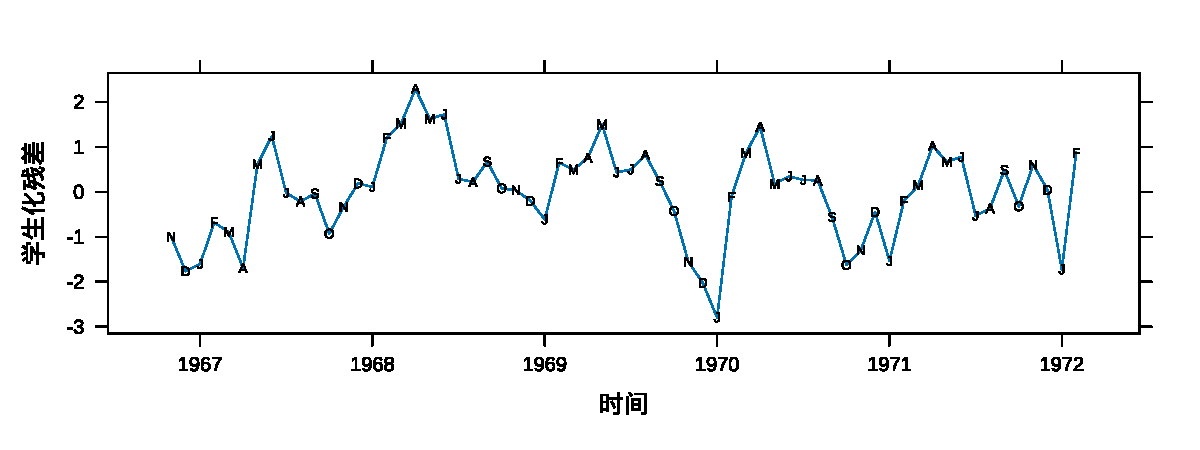
\includegraphics{chapter3_files/figure-latex/winnebago-log-res-1.pdf}
\caption{\label{fig:winnebago-log-res}自然对数变换后的残差图。}
\end{figure}

此图看起来更像是随机噪声(图\ref{fig:winnebago-log-res})。尽管某些月份的值仍有些聚集,但比线性模型已经有了明显的改进。不过我们仍然系统性地高估了某些月份的数值。

\hypertarget{e-2}{%
\subsubsection*{e}\label{e-2}}
\addcontentsline{toc}{subsubsection}{e}

\begin{Shaded}
\begin{Highlighting}[]
\NormalTok{winn\_fit\_seasonal }\OtherTok{\textless{}{-}} \FunctionTok{lm}\NormalTok{(}\FunctionTok{log}\NormalTok{(winnebago) }\SpecialCharTok{\textasciitilde{}} \FunctionTok{season}\NormalTok{(winnebago) }\SpecialCharTok{+} \FunctionTok{time}\NormalTok{(winnebago))}
\FunctionTok{pander}\NormalTok{(}\FunctionTok{summary}\NormalTok{(winn\_fit\_seasonal))}
\end{Highlighting}
\end{Shaded}

\begin{longtable}[]{@{}
  >{\centering\arraybackslash}p{(\columnwidth - 8\tabcolsep) * \real{0.4177}}
  >{\centering\arraybackslash}p{(\columnwidth - 8\tabcolsep) * \real{0.1392}}
  >{\centering\arraybackslash}p{(\columnwidth - 8\tabcolsep) * \real{0.1646}}
  >{\centering\arraybackslash}p{(\columnwidth - 8\tabcolsep) * \real{0.1266}}
  >{\centering\arraybackslash}p{(\columnwidth - 8\tabcolsep) * \real{0.1519}}@{}}
\toprule\noalign{}
\begin{minipage}[b]{\linewidth}\centering
~
\end{minipage} & \begin{minipage}[b]{\linewidth}\centering
Estimate
\end{minipage} & \begin{minipage}[b]{\linewidth}\centering
Std. Error
\end{minipage} & \begin{minipage}[b]{\linewidth}\centering
t value
\end{minipage} & \begin{minipage}[b]{\linewidth}\centering
Pr(\textgreater\textbar t\textbar)
\end{minipage} \\
\midrule\noalign{}
\endhead
\bottomrule\noalign{}
\endlastfoot
\textbf{(Intercept)} & -997.3 & 50.64 & -19.69 & 1.718e-25 \\
\textbf{season(winnebago)February} & 0.6244 & 0.1818 & 3.434 & 0.001188 \\
\textbf{season(winnebago)March} & 0.6822 & 0.1909 & 3.574 & 0.0007793 \\
\textbf{season(winnebago)April} & 0.8096 & 0.1908 & 4.243 & 9.301e-05 \\
\textbf{season(winnebago)May} & 0.8695 & 0.1907 & 4.559 & 3.246e-05 \\
\textbf{season(winnebago)June} & 0.8631 & 0.1907 & 4.526 & 3.627e-05 \\
\textbf{season(winnebago)July} & 0.5539 & 0.1907 & 2.905 & 0.00542 \\
\textbf{season(winnebago)August} & 0.5699 & 0.1907 & 2.988 & 0.004305 \\
\textbf{season(winnebago)September} & 0.5757 & 0.1907 & 3.018 & 0.00396 \\
\textbf{season(winnebago)October} & 0.2635 & 0.1908 & 1.381 & 0.1733 \\
\textbf{season(winnebago)November} & 0.2868 & 0.1819 & 1.577 & 0.1209 \\
\textbf{season(winnebago)December} & 0.248 & 0.1818 & 1.364 & 0.1785 \\
\textbf{time(winnebago)} & 0.5091 & 0.02571 & 19.8 & 1.351e-25 \\
\end{longtable}

\begin{longtable}[]{@{}
  >{\centering\arraybackslash}p{(\columnwidth - 6\tabcolsep) * \real{0.2083}}
  >{\centering\arraybackslash}p{(\columnwidth - 6\tabcolsep) * \real{0.3056}}
  >{\centering\arraybackslash}p{(\columnwidth - 6\tabcolsep) * \real{0.1250}}
  >{\centering\arraybackslash}p{(\columnwidth - 6\tabcolsep) * \real{0.2361}}@{}}
\caption{Fitting linear model: log(winnebago) \textasciitilde{} season(winnebago) + time(winnebago)}\tabularnewline
\toprule\noalign{}
\begin{minipage}[b]{\linewidth}\centering
Observations
\end{minipage} & \begin{minipage}[b]{\linewidth}\centering
Residual Std. Error
\end{minipage} & \begin{minipage}[b]{\linewidth}\centering
\(R^2\)
\end{minipage} & \begin{minipage}[b]{\linewidth}\centering
Adjusted \(R^2\)
\end{minipage} \\
\midrule\noalign{}
\endfirsthead
\toprule\noalign{}
\begin{minipage}[b]{\linewidth}\centering
Observations
\end{minipage} & \begin{minipage}[b]{\linewidth}\centering
Residual Std. Error
\end{minipage} & \begin{minipage}[b]{\linewidth}\centering
\(R^2\)
\end{minipage} & \begin{minipage}[b]{\linewidth}\centering
Adjusted \(R^2\)
\end{minipage} \\
\midrule\noalign{}
\endhead
\bottomrule\noalign{}
\endlastfoot
64 & 0.3149 & 0.8946 & 0.8699 \\
\end{longtable}

通过加入季节性因素进一步提高了模型的拟合度。\(R^2\) 达到0.89,季节性均值以及时间趋势的显著性检验也大多通过。

\hypertarget{f-1}{%
\subsubsection*{f}\label{f-1}}
\addcontentsline{toc}{subsubsection}{f}

\begin{Shaded}
\begin{Highlighting}[]
\FunctionTok{xyplot}\NormalTok{(}\FunctionTok{rstudent}\NormalTok{(winn\_fit\_seasonal) }\SpecialCharTok{\textasciitilde{}} \FunctionTok{time}\NormalTok{(winnebago), }\AttributeTok{type =} \StringTok{"l"}\NormalTok{,}
       \AttributeTok{xlab =} \StringTok{"时间"}\NormalTok{, }\AttributeTok{ylab =} \StringTok{"学生化残差"}\NormalTok{,}
       \AttributeTok{panel =} \ControlFlowTok{function}\NormalTok{(x, y, ...) \{}
         \FunctionTok{panel.xyplot}\NormalTok{(x, y, ...)}
         \FunctionTok{panel.xyplot}\NormalTok{(x, y, }\AttributeTok{col =} \DecValTok{1}\NormalTok{, }\AttributeTok{pch =} \FunctionTok{as.vector}\NormalTok{(}\FunctionTok{season}\NormalTok{(winnebago)))}
\NormalTok{       \})}
\end{Highlighting}
\end{Shaded}

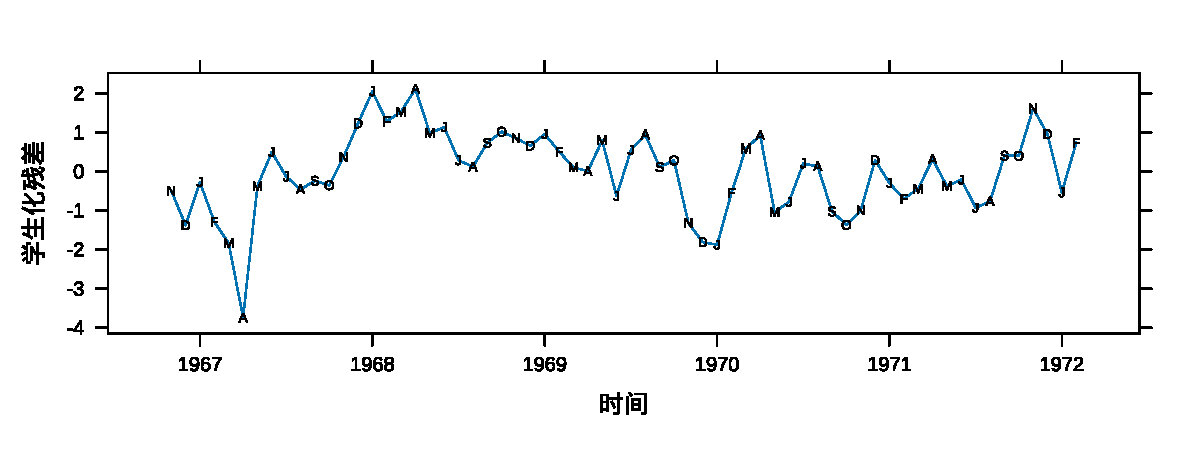
\includegraphics{chapter3_files/figure-latex/winnebago-seasonal-res-1.pdf}

虽然在时间序列开始时某些残差较大,但总体来说模型可以接受(图\ref{fig:winnebago-seasonal-res})。

\hypertarget{ux91cdux65b0ux63a2ux8ba8ux5de5ux4f5cux65f6ux95f4}{%
\subsection{3.10 重新探讨工作时间}\label{ux91cdux65b0ux63a2ux8ba8ux5de5ux4f5cux65f6ux95f4}}

\hypertarget{a-4}{%
\subsubsection*{a}\label{a-4}}
\addcontentsline{toc}{subsubsection}{a}

\begin{Shaded}
\begin{Highlighting}[]
\FunctionTok{data}\NormalTok{(hours)}
\NormalTok{hours\_quad }\OtherTok{\textless{}{-}} \FunctionTok{lm}\NormalTok{(hours }\SpecialCharTok{\textasciitilde{}} \FunctionTok{time}\NormalTok{(hours) }\SpecialCharTok{+} \FunctionTok{I}\NormalTok{(}\FunctionTok{time}\NormalTok{(hours)}\SpecialCharTok{\^{}}\DecValTok{2}\NormalTok{))}
\FunctionTok{pander}\NormalTok{(}\FunctionTok{summary}\NormalTok{(hours\_quad))}
\end{Highlighting}
\end{Shaded}

\begin{longtable}[]{@{}
  >{\centering\arraybackslash}p{(\columnwidth - 8\tabcolsep) * \real{0.3194}}
  >{\centering\arraybackslash}p{(\columnwidth - 8\tabcolsep) * \real{0.1528}}
  >{\centering\arraybackslash}p{(\columnwidth - 8\tabcolsep) * \real{0.1806}}
  >{\centering\arraybackslash}p{(\columnwidth - 8\tabcolsep) * \real{0.1389}}
  >{\centering\arraybackslash}p{(\columnwidth - 8\tabcolsep) * \real{0.1667}}@{}}
\toprule\noalign{}
\begin{minipage}[b]{\linewidth}\centering
~
\end{minipage} & \begin{minipage}[b]{\linewidth}\centering
Estimate
\end{minipage} & \begin{minipage}[b]{\linewidth}\centering
Std. Error
\end{minipage} & \begin{minipage}[b]{\linewidth}\centering
t value
\end{minipage} & \begin{minipage}[b]{\linewidth}\centering
Pr(\textgreater\textbar t\textbar)
\end{minipage} \\
\midrule\noalign{}
\endhead
\bottomrule\noalign{}
\endlastfoot
\textbf{(Intercept)} & -512240 & 115544 & -4.433 & 4.281e-05 \\
\textbf{time(hours)} & 515.9 & 116.4 & 4.431 & 4.314e-05 \\
\textbf{I(time(hours)\^{}2)} & -0.1299 & 0.02933 & -4.428 & 4.353e-05 \\
\end{longtable}

\begin{longtable}[]{@{}
  >{\centering\arraybackslash}p{(\columnwidth - 6\tabcolsep) * \real{0.2083}}
  >{\centering\arraybackslash}p{(\columnwidth - 6\tabcolsep) * \real{0.3056}}
  >{\centering\arraybackslash}p{(\columnwidth - 6\tabcolsep) * \real{0.1250}}
  >{\centering\arraybackslash}p{(\columnwidth - 6\tabcolsep) * \real{0.2361}}@{}}
\caption{Fitting linear model: hours \textasciitilde{} time(hours) + I(time(hours)\^{}2)}\tabularnewline
\toprule\noalign{}
\begin{minipage}[b]{\linewidth}\centering
Observations
\end{minipage} & \begin{minipage}[b]{\linewidth}\centering
Residual Std. Error
\end{minipage} & \begin{minipage}[b]{\linewidth}\centering
\(R^2\)
\end{minipage} & \begin{minipage}[b]{\linewidth}\centering
Adjusted \(R^2\)
\end{minipage} \\
\midrule\noalign{}
\endfirsthead
\toprule\noalign{}
\begin{minipage}[b]{\linewidth}\centering
Observations
\end{minipage} & \begin{minipage}[b]{\linewidth}\centering
Residual Std. Error
\end{minipage} & \begin{minipage}[b]{\linewidth}\centering
\(R^2\)
\end{minipage} & \begin{minipage}[b]{\linewidth}\centering
Adjusted \(R^2\)
\end{minipage} \\
\midrule\noalign{}
\endhead
\bottomrule\noalign{}
\endlastfoot
60 & 0.423 & 0.5921 & 0.5778 \\
\end{longtable}

线性和二次趋势均显著。我们解释了总方差的59\%。

\hypertarget{b-4}{%
\subsubsection*{b}\label{b-4}}
\addcontentsline{toc}{subsubsection}{b}

\begin{Shaded}
\begin{Highlighting}[]
\FunctionTok{xyplot}\NormalTok{(}\FunctionTok{rstudent}\NormalTok{(hours\_quad) }\SpecialCharTok{\textasciitilde{}} \FunctionTok{seq\_along}\NormalTok{(hours), }\AttributeTok{type =} \StringTok{"l"}\NormalTok{,}
       \AttributeTok{xlab =} \StringTok{"指数"}\NormalTok{, }\AttributeTok{ylab =} \StringTok{"学生化残差"}\NormalTok{,}
       \AttributeTok{panel =} \ControlFlowTok{function}\NormalTok{(x, y, ...) \{}
         \FunctionTok{panel.xyplot}\NormalTok{(x, y, ...)}
         \FunctionTok{panel.xyplot}\NormalTok{(x, y, }\AttributeTok{pch =} \FunctionTok{as.vector}\NormalTok{(}\FunctionTok{season}\NormalTok{(hours)), }\AttributeTok{col =} \DecValTok{1}\NormalTok{)}
\NormalTok{       \})}
\end{Highlighting}
\end{Shaded}

\begin{figure}
\centering
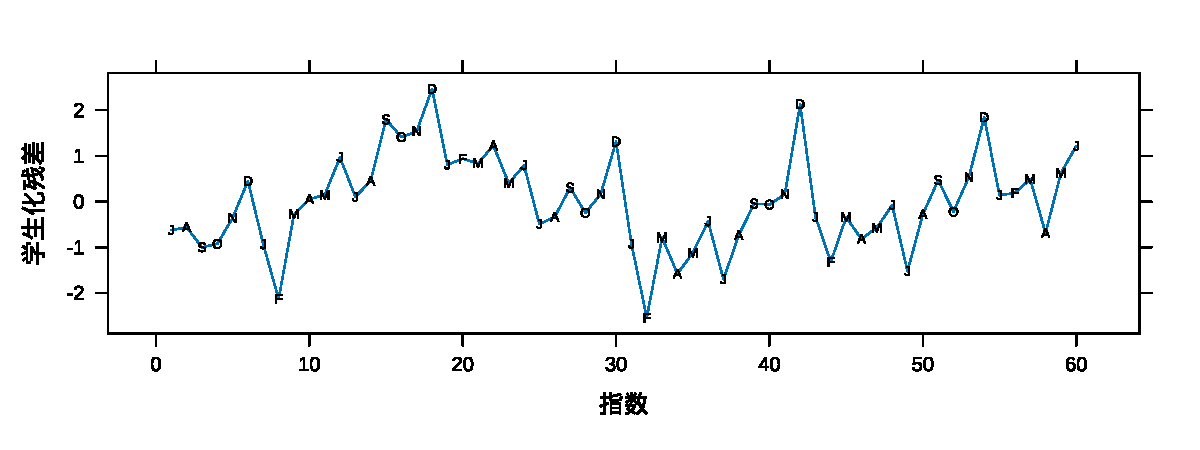
\includegraphics{chapter3_files/figure-latex/hours-quad-res-1.pdf}
\caption{\label{fig:hours-quad-res}对小时数序列二次拟合的学生化残差图}
\end{figure}

此处明显遗漏了季节趋势。例如,低估了2月,高估了12月。

\hypertarget{c-3}{%
\subsubsection*{c}\label{c-3}}
\addcontentsline{toc}{subsubsection}{c}

我们运行\textbf{游程检验}来检查观察值间的依赖关系。

\begin{Shaded}
\begin{Highlighting}[]
\FunctionTok{runs}\NormalTok{(}\FunctionTok{rstudent}\NormalTok{(hours\_quad))}
\end{Highlighting}
\end{Shaded}

\begin{verbatim}
## $pvalue
## [1] 0.00012
## 
## $observed.runs
## [1] 16
## 
## $expected.runs
## [1] 30.96667
## 
## $n1
## [1] 31
## 
## $n2
## [1] 29
## 
## $k
## [1] 0
\end{verbatim}

我们的游程数量多于预期,且在\(p = 0.00012\)水平上具有显著性检验结果,证实了我们在(b)部分的猜想。

\hypertarget{d-3}{%
\subsubsection*{d}\label{d-3}}
\addcontentsline{toc}{subsubsection}{d}

我写的\texttt{lat\_acf}是一个用于绘制自相关函数(ACF)图的自定义函数,并利用了\texttt{TSA}包中的\texttt{acf}函数和\texttt{lattice}包中的\texttt{xyplot}函数。

\begin{Shaded}
\begin{Highlighting}[]
\NormalTok{lat\_acf }\OtherTok{\textless{}{-}} \ControlFlowTok{function}\NormalTok{(x, }\AttributeTok{ci =} \FloatTok{0.95}\NormalTok{, }\AttributeTok{drop.lag.0 =} \ConstantTok{FALSE}\NormalTok{, ...) \{}
\NormalTok{  s }\OtherTok{\textless{}{-}}\NormalTok{ TSA}\SpecialCharTok{::}\FunctionTok{acf}\NormalTok{(x, }\AttributeTok{drop.lag.0 =}\NormalTok{ drop.lag}\FloatTok{.0}\NormalTok{, }\AttributeTok{plot =} \ConstantTok{FALSE}\NormalTok{, ...)}

\NormalTok{  nser }\OtherTok{\textless{}{-}} \FunctionTok{ncol}\NormalTok{(s}\SpecialCharTok{$}\NormalTok{lag)}

\NormalTok{  clim0 }\OtherTok{\textless{}{-}} \FunctionTok{qnorm}\NormalTok{((}\DecValTok{1} \SpecialCharTok{+}\NormalTok{ ci) }\SpecialCharTok{/} \DecValTok{2}\NormalTok{) }\SpecialCharTok{/} \FunctionTok{sqrt}\NormalTok{(s}\SpecialCharTok{$}\NormalTok{n.used)}

\NormalTok{  ylim }\OtherTok{\textless{}{-}} \FunctionTok{range}\NormalTok{(s}\SpecialCharTok{$}\NormalTok{acf[, 1L}\SpecialCharTok{:}\NormalTok{nser, 1L}\SpecialCharTok{:}\NormalTok{nser], }\AttributeTok{na.rm =} \ConstantTok{TRUE}\NormalTok{)}
\NormalTok{  ylim }\OtherTok{\textless{}{-}} \FunctionTok{range}\NormalTok{(}\FunctionTok{c}\NormalTok{(}\SpecialCharTok{{-}}\NormalTok{clim0, clim0, ylim))}


\NormalTok{  lattice}\SpecialCharTok{::}\FunctionTok{xyplot}\NormalTok{(s}\SpecialCharTok{$}\NormalTok{acf }\SpecialCharTok{\textasciitilde{}}\NormalTok{ s}\SpecialCharTok{$}\NormalTok{lag, }\AttributeTok{type =} \StringTok{"h"}\NormalTok{, }\AttributeTok{xlab =} \StringTok{"滞后"}\NormalTok{, }\AttributeTok{ylab =} \StringTok{"自相关函数"}\NormalTok{,}
                  \AttributeTok{ylim =}\NormalTok{ ylim }\SpecialCharTok{*} \FloatTok{1.1}\NormalTok{,}
                  \AttributeTok{panel =} \ControlFlowTok{function}\NormalTok{(x, y, ...) \{}
                    \FunctionTok{panel.abline}\NormalTok{(}\AttributeTok{h =} \FunctionTok{c}\NormalTok{(}\SpecialCharTok{{-}}\NormalTok{clim0, }\DecValTok{0}\NormalTok{, clim0), }\AttributeTok{lty =} \FunctionTok{c}\NormalTok{(}\DecValTok{3}\NormalTok{, }\DecValTok{1}\NormalTok{, }\DecValTok{3}\NormalTok{))}
                    \FunctionTok{panel.xyplot}\NormalTok{(x, y, ...)}
\NormalTok{                  \})}
\NormalTok{\}}
\end{Highlighting}
\end{Shaded}

\begin{Shaded}
\begin{Highlighting}[]
\FunctionTok{lat\_acf}\NormalTok{(}\FunctionTok{rstudent}\NormalTok{(hours\_quad))}
\end{Highlighting}
\end{Shaded}

\begin{figure}
\centering
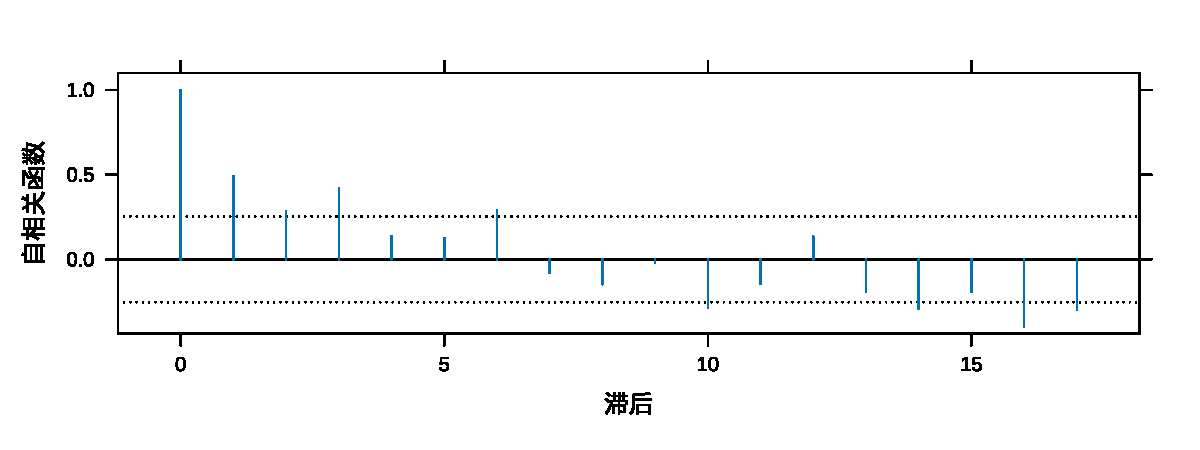
\includegraphics{chapter3_files/figure-latex/hours-acf-1.pdf}
\caption{\label{fig:hours-acf}小时数数据集的自相关图}
\end{figure}

图 \ref{fig:hours-acf} 明确显示了自相关性:前5至6个值之间存在正相关性,之后似乎变为负相关。其中一些值具有显著性。

\hypertarget{e-3}{%
\subsubsection*{e}\label{e-3}}
\addcontentsline{toc}{subsubsection}{e}

\begin{Shaded}
\begin{Highlighting}[]
\NormalTok{figa}\OtherTok{\textless{}{-}}\FunctionTok{qqmath}\NormalTok{(}\FunctionTok{rstudent}\NormalTok{(hours\_quad), }\AttributeTok{asp =} \DecValTok{1}\NormalTok{,}
        \AttributeTok{xlab =} \StringTok{"理论值"}\NormalTok{, }\AttributeTok{ylab =} \StringTok{"学生化残差"}\NormalTok{,}
        \AttributeTok{panel =} \ControlFlowTok{function}\NormalTok{(x, ...) \{}
          \FunctionTok{panel.qqmathline}\NormalTok{(x, ...)}
          \FunctionTok{panel.qqmath}\NormalTok{(x, ...)}
\NormalTok{        \})}
\NormalTok{figb}\OtherTok{\textless{}{-}}\FunctionTok{densityplot}\NormalTok{(}\FunctionTok{rstudent}\NormalTok{(hours\_quad), }\AttributeTok{xlab =} \StringTok{"学生化残差"}\NormalTok{, }
             \AttributeTok{ylab =} \StringTok{"密度"}\NormalTok{)}
\NormalTok{gridExtra}\SpecialCharTok{::}\FunctionTok{grid.arrange}\NormalTok{(figa, figb, }\AttributeTok{ncol =} \DecValTok{2}\NormalTok{)}
\end{Highlighting}
\end{Shaded}

\begin{figure}
\centering
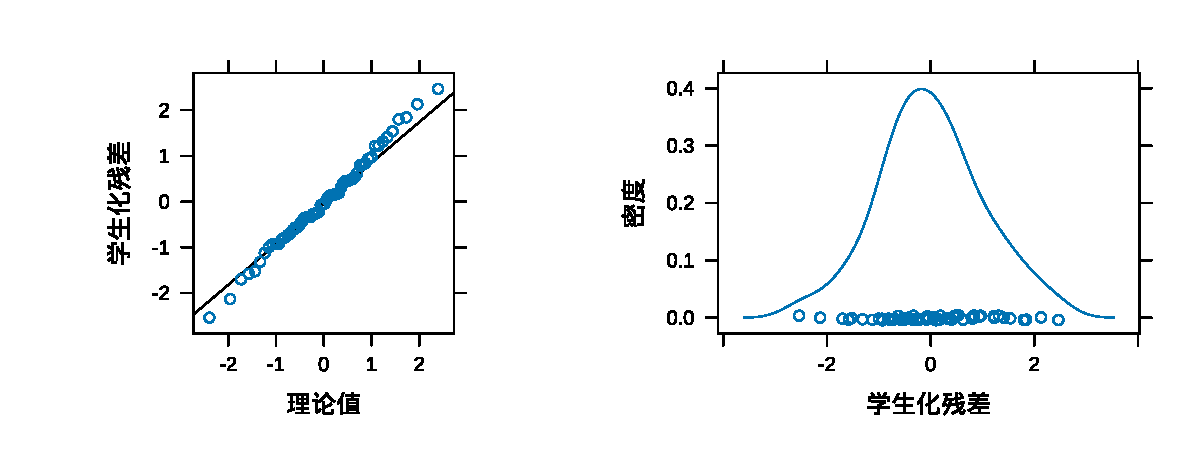
\includegraphics{chapter3_files/figure-latex/normality-test1-1.pdf}
\caption{\label{fig:normality-test1}正态性检验图}
\end{figure}

分布呈现出轻尾特征,但除此之外看起来相当接近正态分布。

\hypertarget{ux91cdux65b0ux63a2ux8ba8ux5de5ux8d44}{%
\subsection{3.11 重新探讨工资}\label{ux91cdux65b0ux63a2ux8ba8ux5de5ux8d44}}

\hypertarget{a-5}{%
\subsubsection*{a}\label{a-5}}
\addcontentsline{toc}{subsubsection}{a}

\begin{Shaded}
\begin{Highlighting}[]
\NormalTok{wages\_quad }\OtherTok{\textless{}{-}} \FunctionTok{lm}\NormalTok{(wages }\SpecialCharTok{\textasciitilde{}} \FunctionTok{time}\NormalTok{(wages) }\SpecialCharTok{+} \FunctionTok{I}\NormalTok{(}\FunctionTok{time}\NormalTok{(wages)}\SpecialCharTok{\^{}}\DecValTok{2}\NormalTok{))}
\FunctionTok{pander}\NormalTok{(}\FunctionTok{summary}\NormalTok{(wages\_quad))}
\end{Highlighting}
\end{Shaded}

\begin{longtable}[]{@{}
  >{\centering\arraybackslash}p{(\columnwidth - 8\tabcolsep) * \real{0.3194}}
  >{\centering\arraybackslash}p{(\columnwidth - 8\tabcolsep) * \real{0.1528}}
  >{\centering\arraybackslash}p{(\columnwidth - 8\tabcolsep) * \real{0.1806}}
  >{\centering\arraybackslash}p{(\columnwidth - 8\tabcolsep) * \real{0.1389}}
  >{\centering\arraybackslash}p{(\columnwidth - 8\tabcolsep) * \real{0.1667}}@{}}
\toprule\noalign{}
\begin{minipage}[b]{\linewidth}\centering
~
\end{minipage} & \begin{minipage}[b]{\linewidth}\centering
Estimate
\end{minipage} & \begin{minipage}[b]{\linewidth}\centering
Std. Error
\end{minipage} & \begin{minipage}[b]{\linewidth}\centering
t value
\end{minipage} & \begin{minipage}[b]{\linewidth}\centering
Pr(\textgreater\textbar t\textbar)
\end{minipage} \\
\midrule\noalign{}
\endhead
\bottomrule\noalign{}
\endlastfoot
\textbf{(Intercept)} & -84950 & 10191 & -8.336 & 4.865e-12 \\
\textbf{time(wages)} & 85.34 & 10.27 & 8.309 & 5.439e-12 \\
\textbf{I(time(wages)\^{}2)} & -0.02143 & 0.002588 & -8.282 & 6.104e-12 \\
\end{longtable}

\begin{longtable}[]{@{}
  >{\centering\arraybackslash}p{(\columnwidth - 6\tabcolsep) * \real{0.2083}}
  >{\centering\arraybackslash}p{(\columnwidth - 6\tabcolsep) * \real{0.3056}}
  >{\centering\arraybackslash}p{(\columnwidth - 6\tabcolsep) * \real{0.1250}}
  >{\centering\arraybackslash}p{(\columnwidth - 6\tabcolsep) * \real{0.2361}}@{}}
\caption{Fitting linear model: wages \textasciitilde{} time(wages) + I(time(wages)\^{}2)}\tabularnewline
\toprule\noalign{}
\begin{minipage}[b]{\linewidth}\centering
Observations
\end{minipage} & \begin{minipage}[b]{\linewidth}\centering
Residual Std. Error
\end{minipage} & \begin{minipage}[b]{\linewidth}\centering
\(R^2\)
\end{minipage} & \begin{minipage}[b]{\linewidth}\centering
Adjusted \(R^2\)
\end{minipage} \\
\midrule\noalign{}
\endfirsthead
\toprule\noalign{}
\begin{minipage}[b]{\linewidth}\centering
Observations
\end{minipage} & \begin{minipage}[b]{\linewidth}\centering
Residual Std. Error
\end{minipage} & \begin{minipage}[b]{\linewidth}\centering
\(R^2\)
\end{minipage} & \begin{minipage}[b]{\linewidth}\centering
Adjusted \(R^2\)
\end{minipage} \\
\midrule\noalign{}
\endhead
\bottomrule\noalign{}
\endlastfoot
72 & 0.05889 & 0.9864 & 0.986 \\
\end{longtable}

这个二次拟合解释了大量的方差(0.99)。

\hypertarget{b-5}{%
\subsubsection*{b}\label{b-5}}
\addcontentsline{toc}{subsubsection}{b}

\begin{Shaded}
\begin{Highlighting}[]
\FunctionTok{runs}\NormalTok{(}\FunctionTok{rstudent}\NormalTok{(wages\_quad))}
\end{Highlighting}
\end{Shaded}

\begin{verbatim}
## $pvalue
## [1] 1.56e-07
## 
## $observed.runs
## [1] 15
## 
## $expected.runs
## [1] 36.75
## 
## $n1
## [1] 33
## 
## $n2
## [1] 39
## 
## $k
## [1] 0
\end{verbatim}

然而,从游程检验的结果可以看出,变量之间存在相互依赖的证据。

\hypertarget{c-4}{%
\subsubsection*{c}\label{c-4}}
\addcontentsline{toc}{subsubsection}{c}

\begin{Shaded}
\begin{Highlighting}[]
\FunctionTok{lat\_acf}\NormalTok{(}\FunctionTok{rstudent}\NormalTok{(wages\_quad))}
\end{Highlighting}
\end{Shaded}

\begin{figure}
\centering
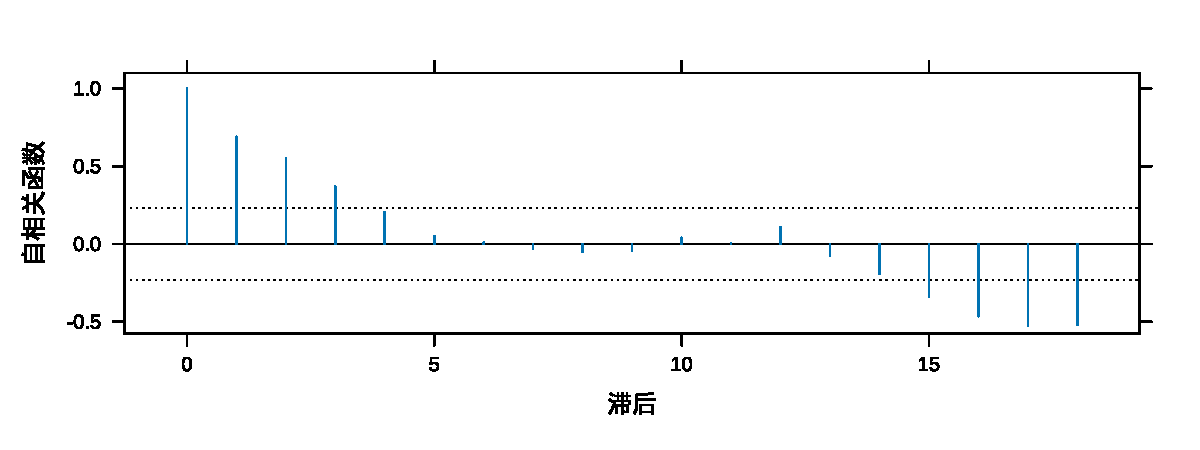
\includegraphics{chapter3_files/figure-latex/wages_acf-1.pdf}
\caption{(\#fig:wages\_acf)基于工资时间序列二次拟合的自相关图}
\end{figure}

但是,自相关图(图@ref(fig:wages\_acf))清楚地表明,我们面临着大量的自相关性,显然这是因为我们尚未考虑该时间序列中的季节性趋势。

\hypertarget{d-4}{%
\subsubsection*{d}\label{d-4}}
\addcontentsline{toc}{subsubsection}{d}

我们也来看看正态性检验图。

\begin{Shaded}
\begin{Highlighting}[]
\NormalTok{figa }\OtherTok{\textless{}{-}} 
  \FunctionTok{qqmath}\NormalTok{(}\FunctionTok{rstudent}\NormalTok{(wages\_quad), }\AttributeTok{xlab =} \StringTok{"理论值"}\NormalTok{,}
       \AttributeTok{asp =} \DecValTok{1}\NormalTok{,}
       \AttributeTok{ylab =} \StringTok{"学生化残差"}\NormalTok{,}
       \AttributeTok{panel =} \ControlFlowTok{function}\NormalTok{(x, ...) \{}
         \FunctionTok{panel.qqmathline}\NormalTok{(x, ...)}
         \FunctionTok{panel.qqmath}\NormalTok{(x, ...)}
\NormalTok{       \})}

\NormalTok{figb }\OtherTok{\textless{}{-}} \FunctionTok{densityplot}\NormalTok{(}\FunctionTok{rstudent}\NormalTok{(wages\_quad), }\AttributeTok{xlab =} \StringTok{"学生化残差"}\NormalTok{,}\AttributeTok{ylab=}\StringTok{"密度"}\NormalTok{)}
\NormalTok{gridExtra}\SpecialCharTok{::}\FunctionTok{grid.arrange}\NormalTok{(figa, figb, }\AttributeTok{ncol =} \DecValTok{2}\NormalTok{)}
\end{Highlighting}
\end{Shaded}

\begin{figure}
\centering
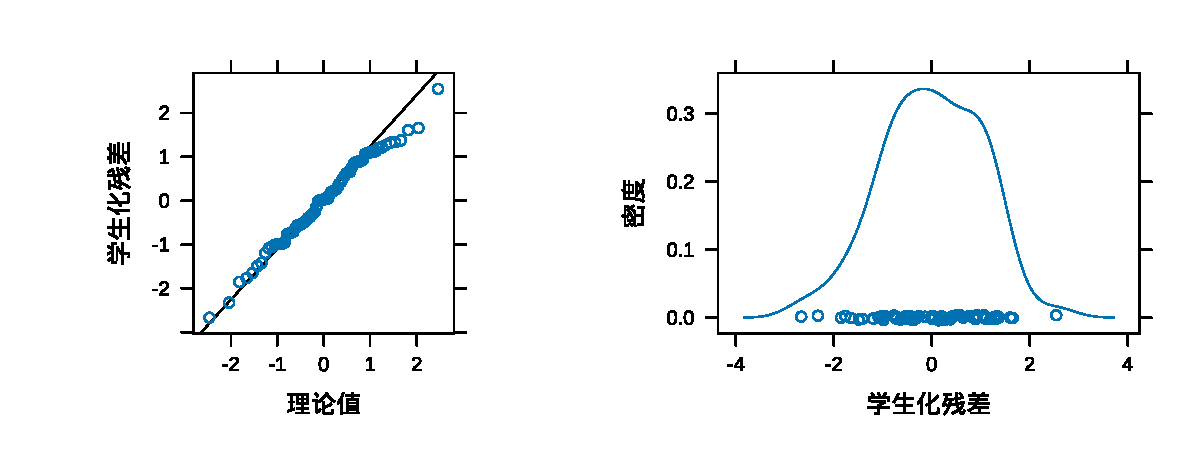
\includegraphics{chapter3_files/figure-latex/wages-norm-1.pdf}
\caption{\label{fig:wages-norm}采用二次拟合的工资数据正态性检验图}
\end{figure}

正态性检验图(图\ref{fig:wages-norm})表明,残差分布具有一定的重尾性,且略微左偏。

\hypertarget{ux91cdux65b0ux63a2ux8ba8ux5564ux9152ux9500ux91cf}{%
\subsection{3.12 重新探讨啤酒销量}\label{ux91cdux65b0ux63a2ux8ba8ux5564ux9152ux9500ux91cf}}

\hypertarget{a-6}{%
\subsubsection*{a}\label{a-6}}
\addcontentsline{toc}{subsubsection}{a}

首先,我们收集残差。

\begin{Shaded}
\begin{Highlighting}[]
\CommentTok{\# 加载数据集(beersales)}
\NormalTok{beer\_quad\_seasonal }\OtherTok{\textless{}{-}} \FunctionTok{lm}\NormalTok{(beersales }\SpecialCharTok{\textasciitilde{}} \FunctionTok{time}\NormalTok{(beersales) }\SpecialCharTok{+} \FunctionTok{I}\NormalTok{(}\FunctionTok{time}\NormalTok{(beersales)}\SpecialCharTok{\^{}}\DecValTok{2}\NormalTok{) }\SpecialCharTok{+}
                           \FunctionTok{season}\NormalTok{(beersales))}
\NormalTok{beer\_resid }\OtherTok{\textless{}{-}} \FunctionTok{rstudent}\NormalTok{(beer\_quad\_seasonal)}
\end{Highlighting}
\end{Shaded}

\hypertarget{b-6}{%
\subsubsection*{b}\label{b-6}}
\addcontentsline{toc}{subsubsection}{b}

接下来,我们执行一次游程检验。

\begin{Shaded}
\begin{Highlighting}[]
\FunctionTok{runs}\NormalTok{(beer\_resid)}
\end{Highlighting}
\end{Shaded}

\begin{verbatim}
## $pvalue
## [1] 0.0127
## 
## $observed.runs
## [1] 79
## 
## $expected.runs
## [1] 96.625
## 
## $n1
## [1] 90
## 
## $n2
## [1] 102
## 
## $k
## [1] 0
\end{verbatim}

检验结果显著(\(p = 0.0127\))。

\hypertarget{c-5}{%
\subsubsection*{c}\label{c-5}}
\addcontentsline{toc}{subsubsection}{c}

\begin{Shaded}
\begin{Highlighting}[]
\FunctionTok{lat\_acf}\NormalTok{(beer\_resid)}
\end{Highlighting}
\end{Shaded}

\begin{figure}
\centering
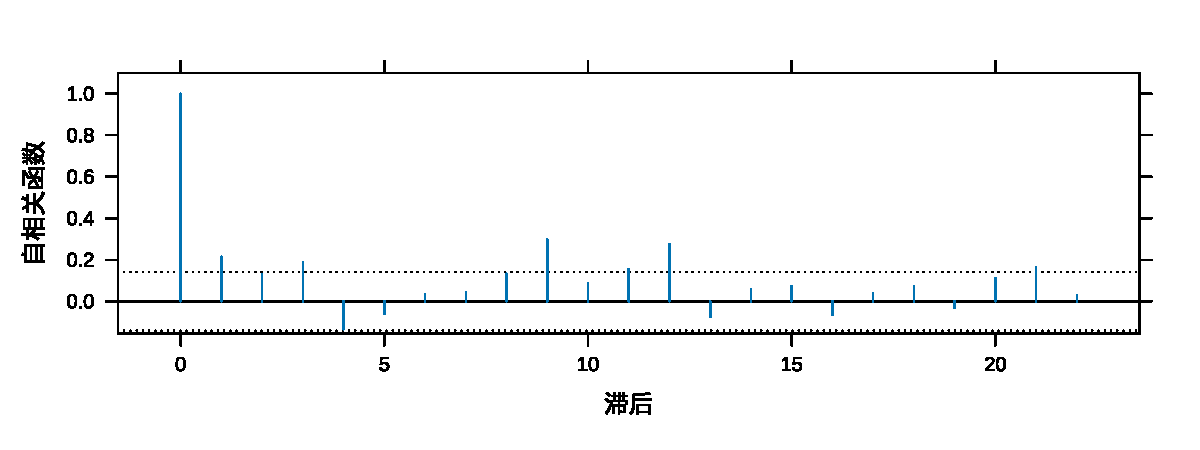
\includegraphics{chapter3_files/figure-latex/beer-acf-1.pdf}
\caption{\label{fig:beer-acf}啤酒销量模型的自相关图}
\end{figure}

因为在几个滞后期上相关性显著,这让我们质疑数据的独立性。

\hypertarget{d-5}{%
\subsubsection*{d}\label{d-5}}
\addcontentsline{toc}{subsubsection}{d}

\begin{Shaded}
\begin{Highlighting}[]
\NormalTok{figa }\OtherTok{\textless{}{-}} 
  \FunctionTok{qqmath}\NormalTok{(beer\_resid, }\AttributeTok{xlab =} \StringTok{"理论值"}\NormalTok{,}
       \AttributeTok{asp =} \DecValTok{1}\NormalTok{,}
       \AttributeTok{ylab =} \StringTok{"学生化残差"}\NormalTok{,}
       \AttributeTok{panel =} \ControlFlowTok{function}\NormalTok{(x, ...) \{}
         \FunctionTok{panel.qqmathline}\NormalTok{(x, ...)}
         \FunctionTok{panel.qqmath}\NormalTok{(x, ...)}
\NormalTok{       \})}

\NormalTok{figb }\OtherTok{\textless{}{-}} \FunctionTok{densityplot}\NormalTok{(beer\_resid, }\AttributeTok{xlab =} \StringTok{"学生化残差"}\NormalTok{)}

\NormalTok{gridExtra}\SpecialCharTok{::}\FunctionTok{grid.arrange}\NormalTok{(figa, figb, }\AttributeTok{ncol =} \DecValTok{2}\NormalTok{)}
\end{Highlighting}
\end{Shaded}

\begin{figure}
\centering
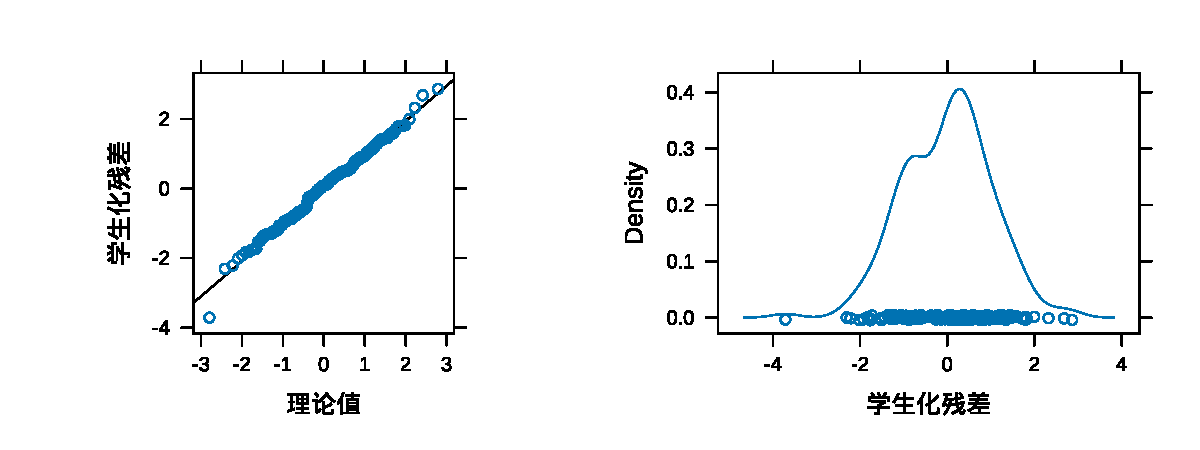
\includegraphics{chapter3_files/figure-latex/beer-norm-1.pdf}
\caption{\label{fig:beer-norm}经过线性、二次及季节性拟合后的啤酒销量时间序列正态性检验图。}
\end{figure}

\hypertarget{ux91cdux65b0ux63a2ux8ba8ux6e29ux5c3cux8d1dux6208ux623fux8f66ux6570ux636e}{%
\subsection{3.13 重新探讨温尼贝戈房车数据}\label{ux91cdux65b0ux63a2ux8ba8ux6e29ux5c3cux8d1dux6208ux623fux8f66ux6570ux636e}}

\hypertarget{a-7}{%
\subsubsection*{a}\label{a-7}}
\addcontentsline{toc}{subsubsection}{a}

\begin{Shaded}
\begin{Highlighting}[]
\NormalTok{winn\_resid }\OtherTok{\textless{}{-}} \FunctionTok{rstudent}\NormalTok{(winn\_fit\_seasonal)}
\end{Highlighting}
\end{Shaded}

\hypertarget{b-7}{%
\subsubsection*{b}\label{b-7}}
\addcontentsline{toc}{subsubsection}{b}

\begin{Shaded}
\begin{Highlighting}[]
\FunctionTok{runs}\NormalTok{(winn\_resid)}
\end{Highlighting}
\end{Shaded}

\begin{verbatim}
## $pvalue
## [1] 0.000243
## 
## $observed.runs
## [1] 18
## 
## $expected.runs
## [1] 32.71875
## 
## $n1
## [1] 29
## 
## $n2
## [1] 35
## 
## $k
## [1] 0
\end{verbatim}

游程检验结果显著。我们得到的游程数目少于预期。

\hypertarget{c-6}{%
\subsubsection*{c}\label{c-6}}
\addcontentsline{toc}{subsubsection}{c}

\begin{Shaded}
\begin{Highlighting}[]
\FunctionTok{lat\_acf}\NormalTok{(winn\_resid)}
\end{Highlighting}
\end{Shaded}

\begin{figure}
\centering
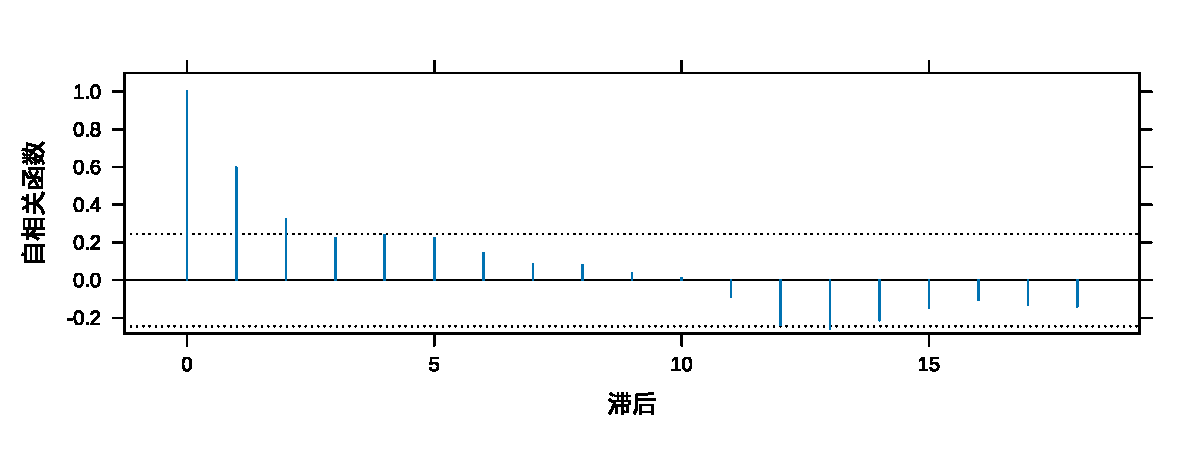
\includegraphics{chapter3_files/figure-latex/winn-acf-1.pdf}
\caption{\label{fig:winn-acf}温尼贝戈房车模型的自相关图。}
\end{figure}

存在依赖性证据,而目前我们在模型中尚未考虑这一因素。

\hypertarget{d-6}{%
\subsubsection*{d}\label{d-6}}
\addcontentsline{toc}{subsubsection}{d}

\begin{Shaded}
\begin{Highlighting}[]
\NormalTok{figa }\OtherTok{\textless{}{-}} 
  \FunctionTok{qqmath}\NormalTok{(winn\_resid, }\AttributeTok{xlab =} \StringTok{"理论值"}\NormalTok{,}
       \AttributeTok{asp =} \DecValTok{1}\NormalTok{,}
       \AttributeTok{ylab =} \StringTok{"学生化残差"}\NormalTok{,}
       \AttributeTok{panel =} \ControlFlowTok{function}\NormalTok{(x, ...) \{}
         \FunctionTok{panel.qqmathline}\NormalTok{(x, ...)}
         \FunctionTok{panel.qqmath}\NormalTok{(x, ...)}
\NormalTok{       \})}

\NormalTok{figb }\OtherTok{\textless{}{-}} \FunctionTok{densityplot}\NormalTok{(winn\_resid, }\AttributeTok{xlab =} \StringTok{"学生化残差"}\NormalTok{,}\AttributeTok{ylab=}\StringTok{"密度"}\NormalTok{)}
\NormalTok{gridExtra}\SpecialCharTok{::}\FunctionTok{grid.arrange}\NormalTok{(figa, figb, }\AttributeTok{ncol =} \DecValTok{2}\NormalTok{)}
\end{Highlighting}
\end{Shaded}

\begin{figure}
\centering
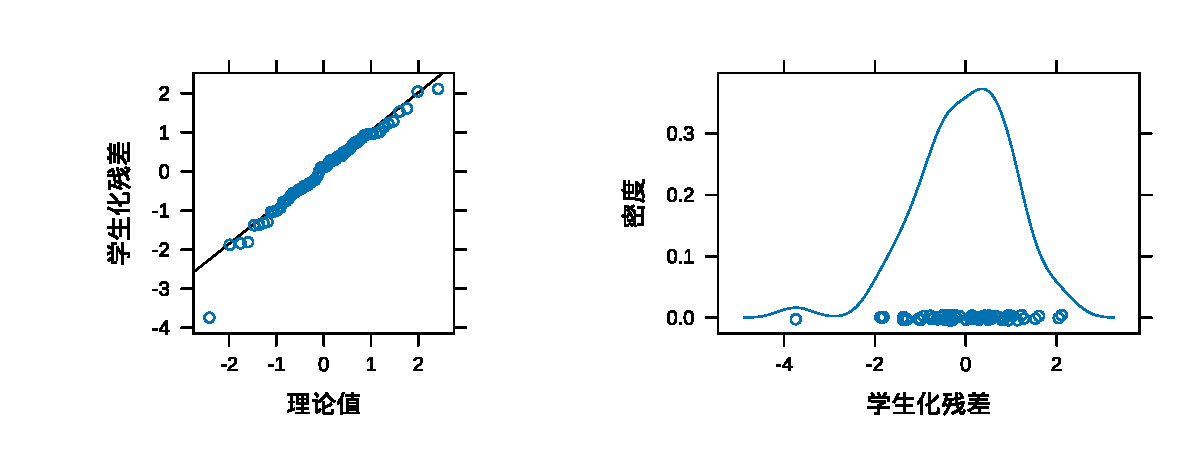
\includegraphics{chapter3_files/figure-latex/winn-norm-1.pdf}
\caption{\label{fig:winn-norm}经过对数变换和季节性拟合后温尼贝戈房车系列的正态性检验图}
\end{figure}

存在左偏斜现象,且有一个较大的异常值,但总体上接近正态分布。

\end{document}
